% chap2.tex
\part{프로그램 구성}
\label{part:ioref}

% ---------------------------------------------------------------------------- %
%                                  NEW SECTION                                 %
% ---------------------------------------------------------------------------- %

\chapter{프로그램 구성 요소}
본 시뮬레이터 엔진은 핵심 python 모듈(\pymodule)\을 중심으로 개발되었다. 이 시뮬레이터는 Python(3.12)\cite{python312}\과 EnergyPlus(24-2-0)\cite{energyplus242}\를 별도 설치 없이 실행할 수 있도록 패키징되어, 사용자가 어떤 환경에서도 단독으로 실행 할 수 있는 독립형 실행 환경을 제공한다(Figure \ref{fig:package_structure}). 개발한 python 모듈(\pymodule)에 대한 자세한 내용은 후속 장에서 설명한다.

\begin{defaultfigure}
  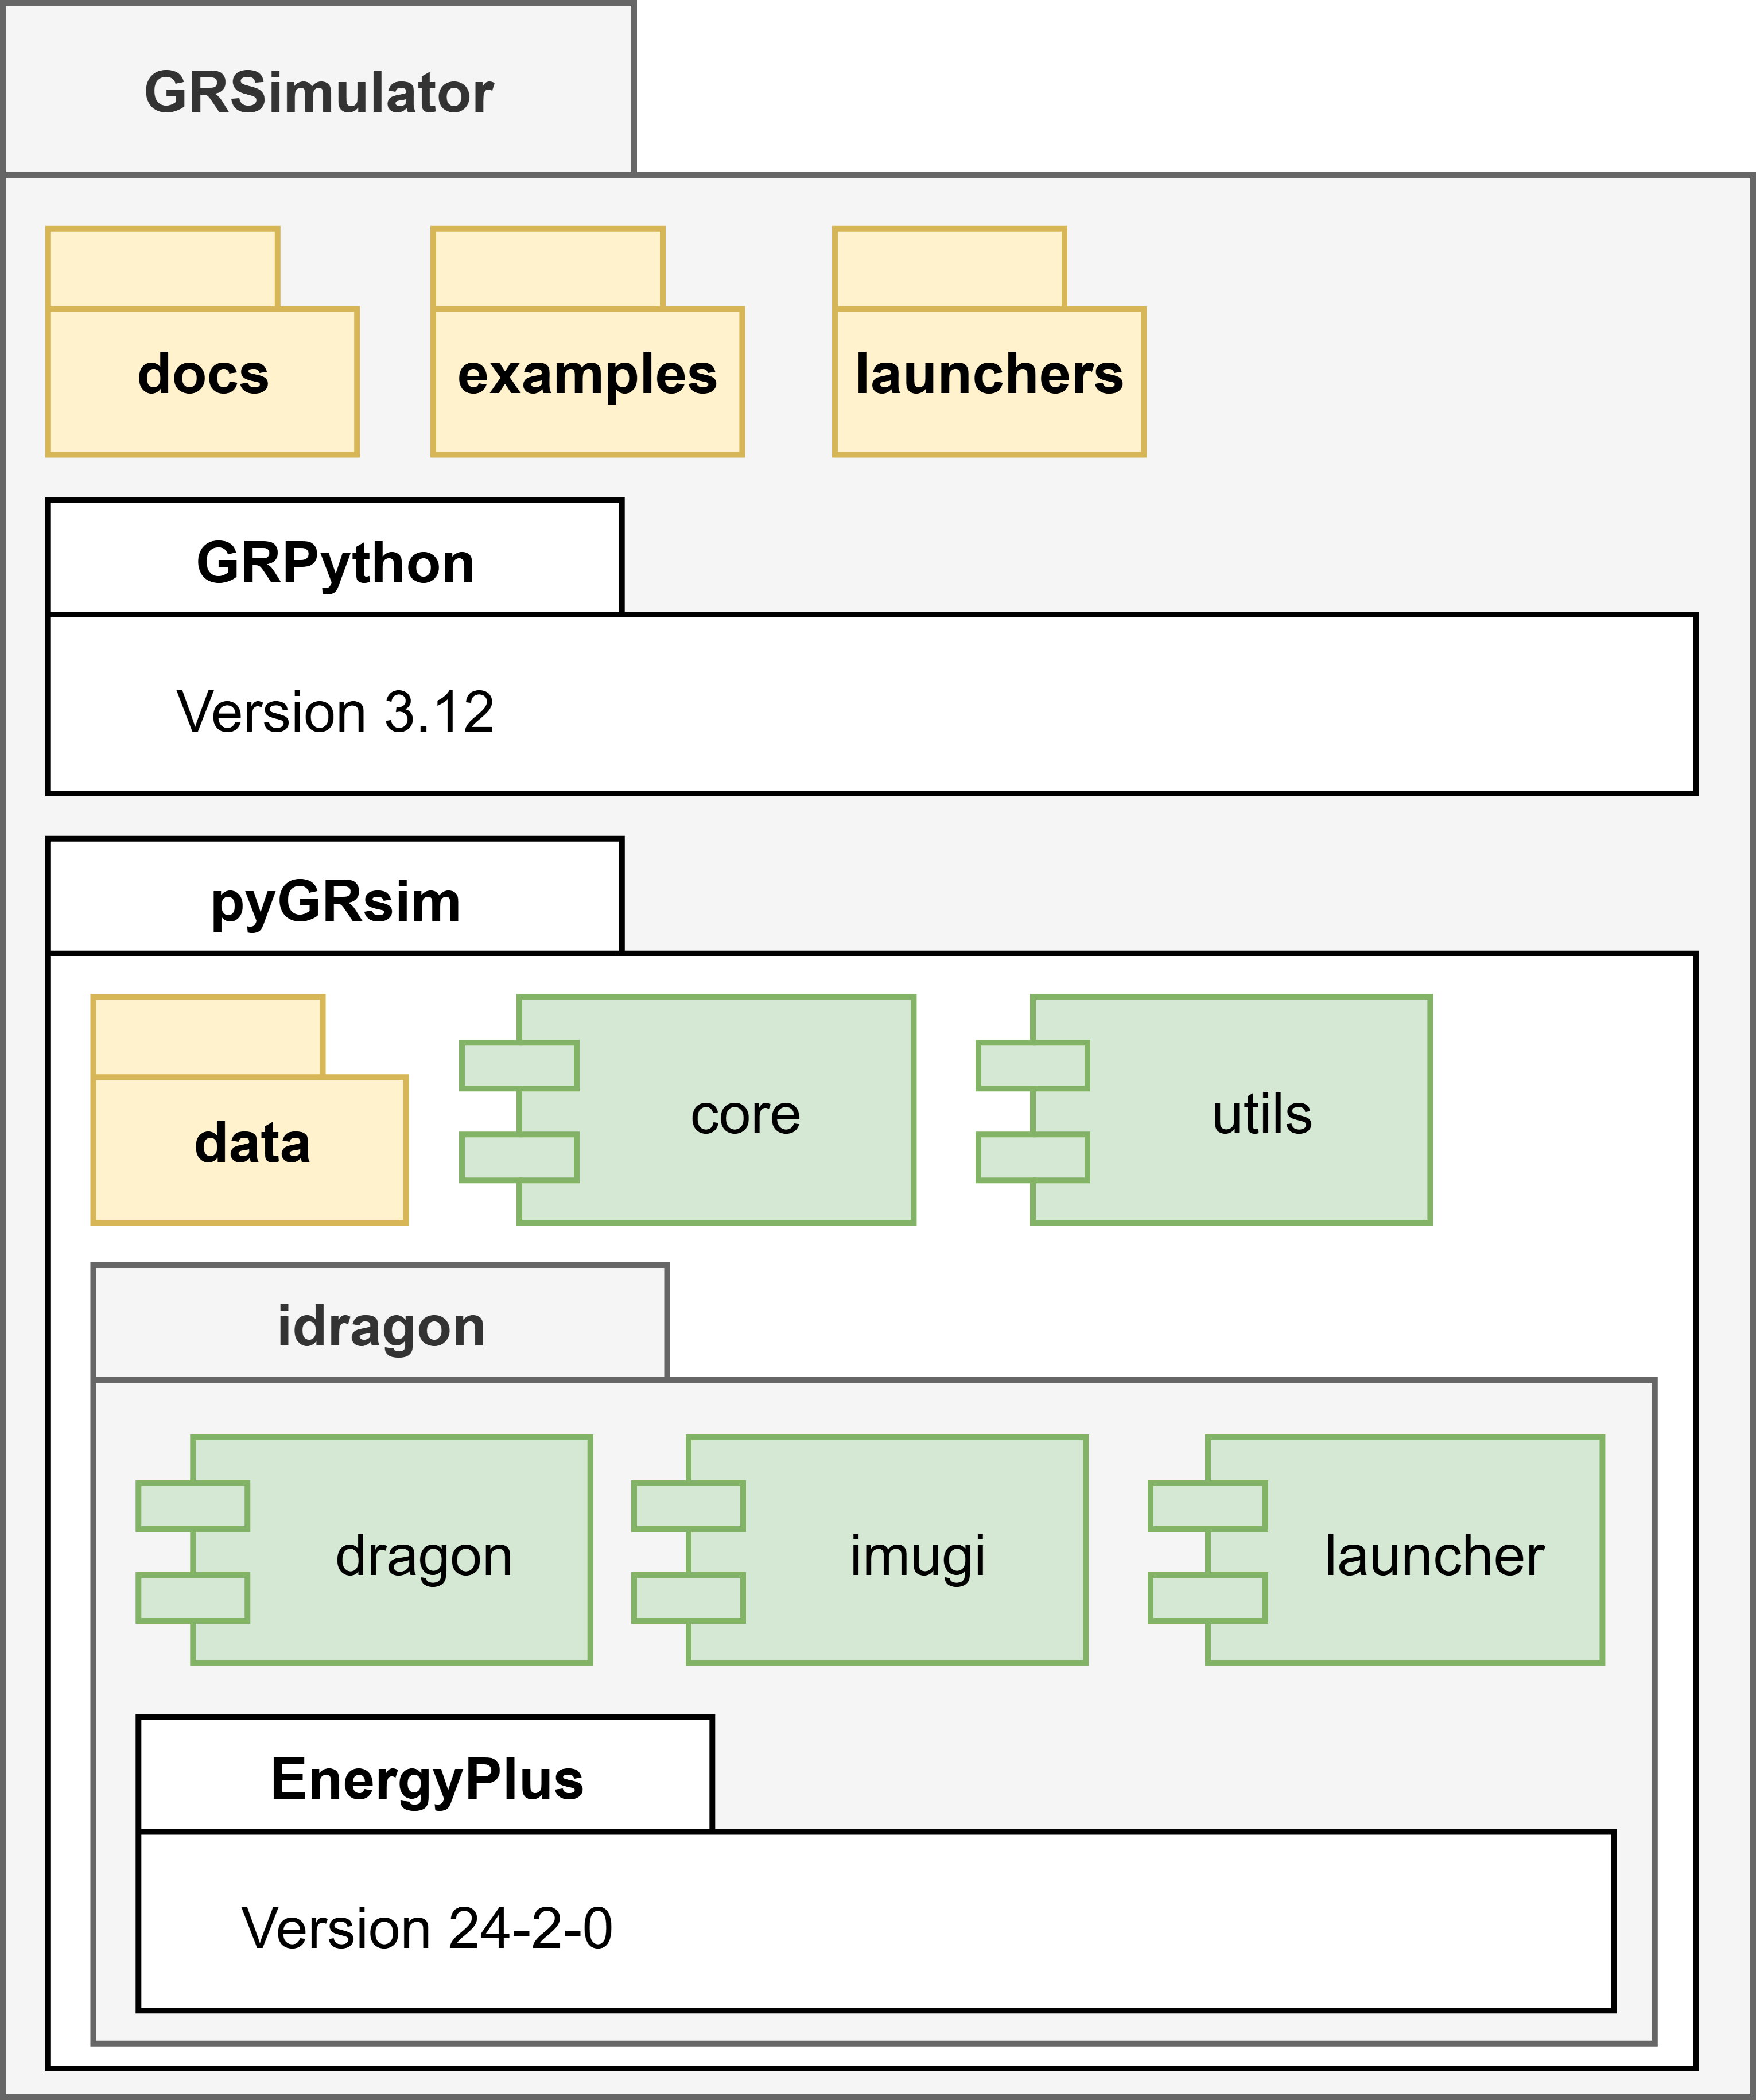
\includegraphics[scale=0.1]{package_structure.png}
  \caption{\simulator\ 프로그램 구조도}
  \label{fig:package_structure}
\end{defaultfigure}

\section{외부 프로그램}

% ---------------------------------------------------------------------------- %
%                                  NEW SECTION                                 %
% ---------------------------------------------------------------------------- %

\subsection{Python 및 그 모듈}
\texttt{Python 3.12} 이용하였다.
데이터 처리 및 연산을 위해 \texttt{pandas}와 \texttt{numpy} 라이브러리를 사용한다.

\subsection{EnergyPlus}
본 시뮬레이터는 \texttt{EnergyPlus 24.2} 버전에 맞추어 개발되었다. \ep는 버전의 상위/하위 호환 모두 지원하지 않으므로, 정확한 버전의 \ep를 요구한다.
참고로, EnergyPlus가 기본 설치 경로(C:/EnergyPlusV24-2-0)에 이미 설치되어 있는 경우, 별도의 패키징 없이도 python 모듈이 해당 경로를 자동으로 찾아 실행할 수 있다. 본 엔진에서 실행 가능한 \ep 찾는 순서는 아래와 같다.

\begin{enumerate}
  \item idragon 모듈 하위의 EnergyPlus 디렉토리
  \item C드라이브에 있는 기본 설치 디렉토리
\end{enumerate}

% ---------------------------------------------------------------------------- %
%                                  NEW SECTION                                 %
% ---------------------------------------------------------------------------- %

\section{예시파일 및 문서}

아래와 같은 문서가 준비되어 있다.
\begin{itemize}
  \item 이 문서랑 별개로 PPT로 만든 사용자 매뉴얼이 제공된다.
  \item 이 문서는 개발자, 연구자용이다.
  \item 개발 과정을 담은 보고서는 ...에 공개되어있으니 참고 가능하다.
\end{itemize}

예시파일들도 준비되어있다. 표준입력과 출력을 n개 건물에 대하여 준비하였다.
\begin{itemize}
  \item grjson   예시도 준비되어있다 (어떤 건물, 어떤 예시).
  \item grexcel  예시도 준비되어있다 (어떤 건물, 어떤 예시).
  \item grresult 예시도 준비되어있다 (어떤 건물, 어떤 예시).
\end{itemize}

% ---------------------------------------------------------------------------- %
%                                  NEW SECTION                                 %
% ---------------------------------------------------------------------------- %

\section{보조 프로그램들}
...하여 실행 가능하다.

\subsection{grexcel 실행 launcher}
RUN\_GREXCEL.bat 파일 실행하면 아래와 같은 창을 확인 가능하다 (Figure \ref{fig:grjson_launcher_capture}).

\begin{defaultfigure}
  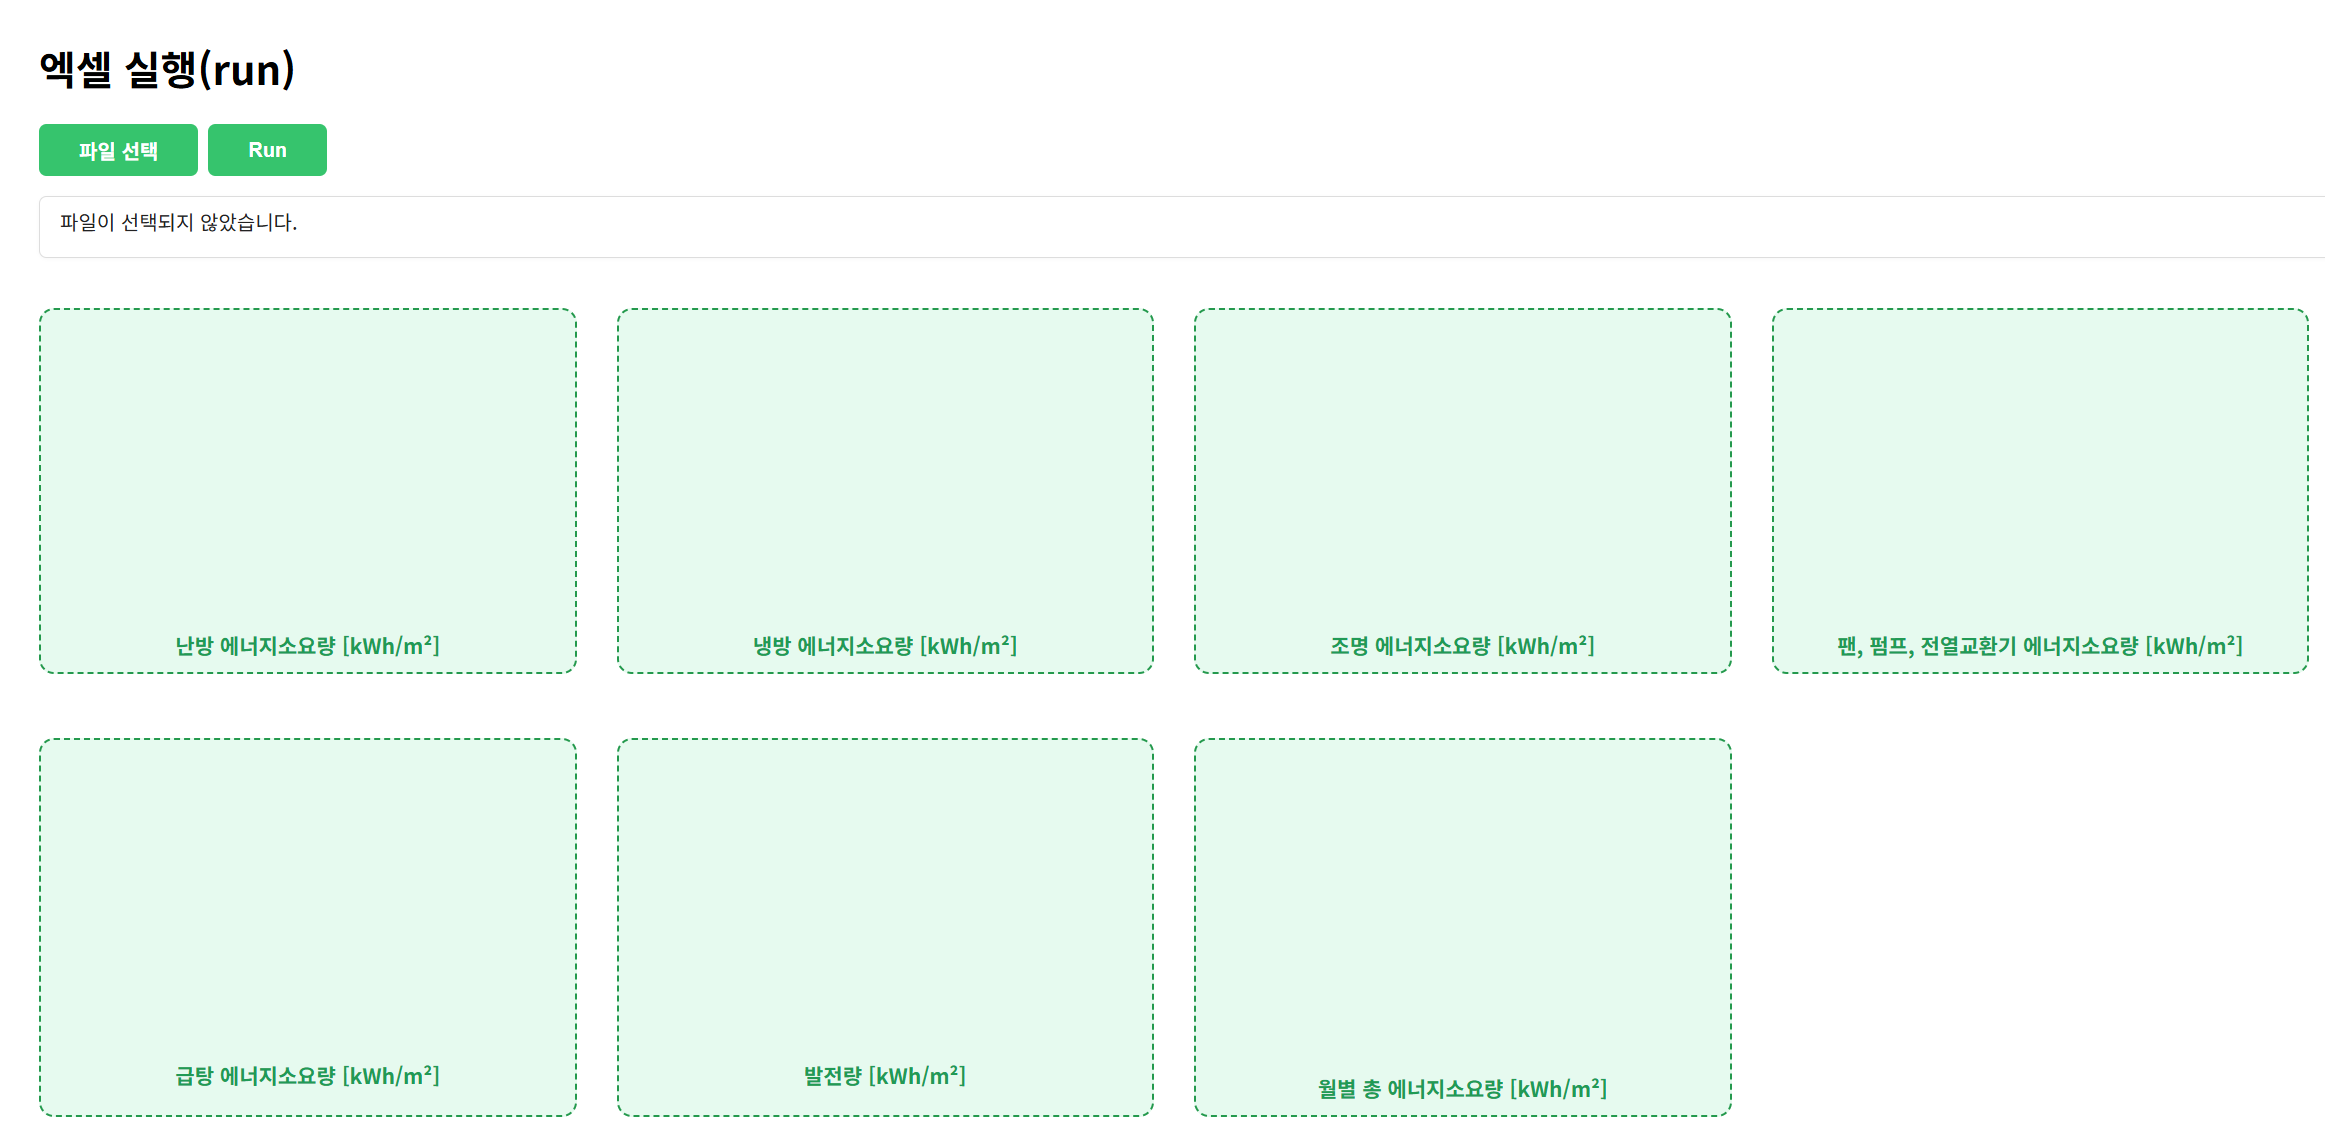
\includegraphics[width=\textwidth]{grexcel launcher 캡처.png}
  \caption{grexcel runner 실행하면 나오는 페이지 (시뮬레이션 전)}
  \label{fig:grjson_launcher_capture}
\end{defaultfigure}

파일 선택하고 run 누르면 백그라운드에서 \simulator가 실행된다. 시뮬레이션이 완료되면, 아래와 같은 창을 확인 가능하다 (Figure \ref{fig:grjson_launcher_capture_result}).

\begin{defaultfigure}
  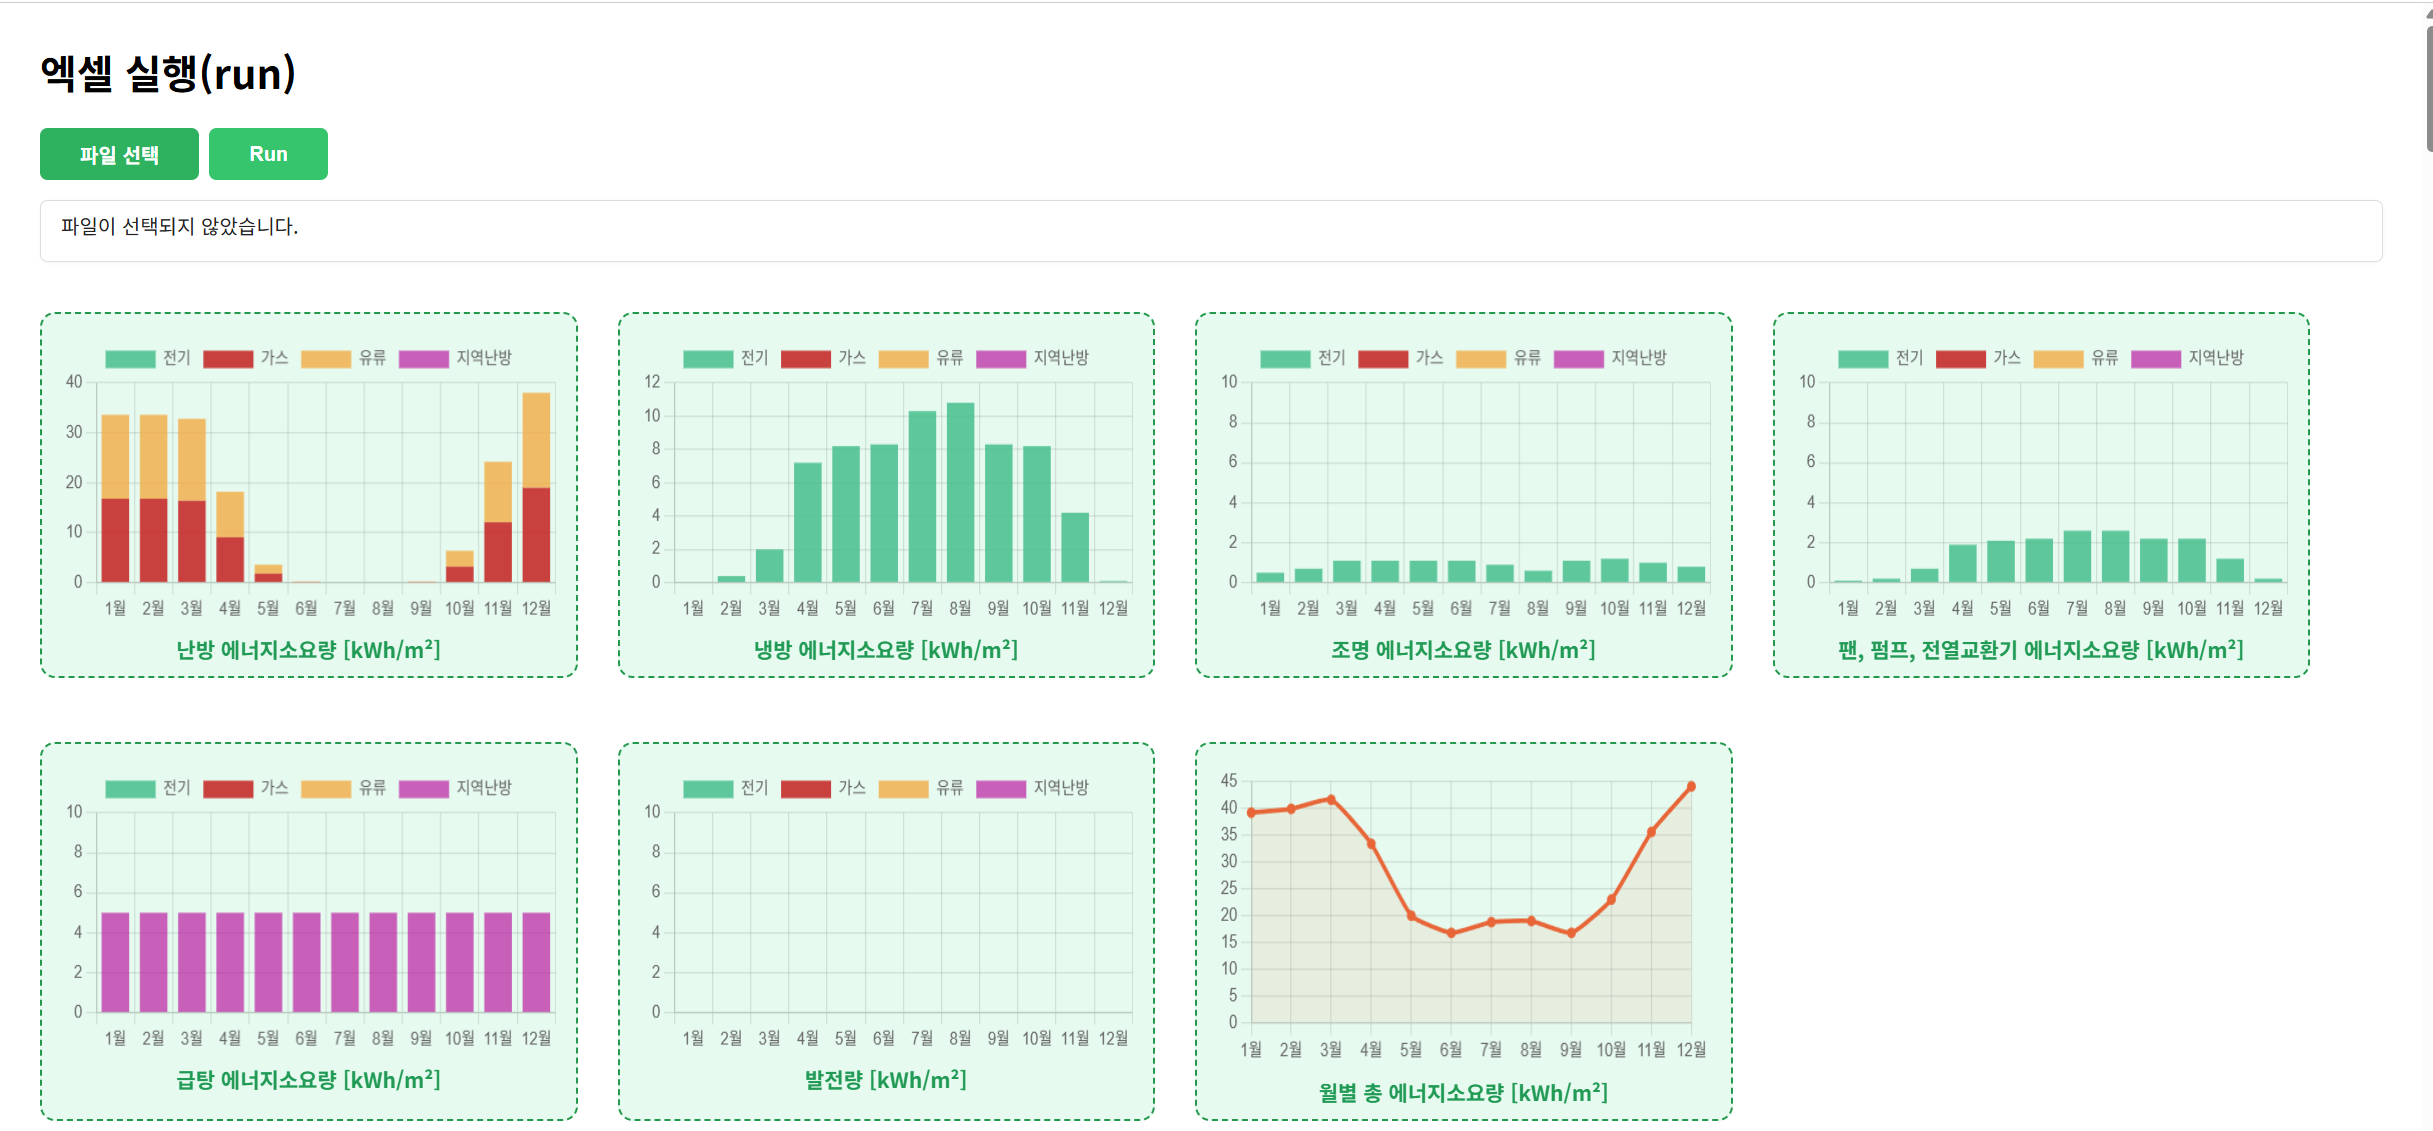
\includegraphics[width=\textwidth]{grexcel launcher 캡처 (결과).png}
  \caption{grexcel runner 실행하면 나오는 페이지 (시뮬레이션 후)}
  \label{fig:grjson_launcher_capture_result}
\end{defaultfigure}


% ---------------------------------------------------------------------------- %
%                                  NEW SECTION                                 %
% ---------------------------------------------------------------------------- %

\section{api}
\subsection{python 모듈의 실행 구조}
표준적인 python 호출 구문은 python -m 모듈이름 *args **kwargs이다. 본 엔진도 동일하다.
runEngine.bat 파일에서 이를 wrap하고 있으니, 이 파일로도 실행이 가능하다.

\subsection{주요 api}

\subsubsection{run: grjson 또는 grexcel 실행}
호출하면 입력파일을 실행한다. 인자는 -i 또는 --input, -o 또는 --output 등 있다. 예시는 아래 코드를 참고.
\begin{tcolorbox}[colback=gray!10, colframe=gray!80, boxrule=0.5pt, left=1em, right=1em]
GRPython/python.exe -m pyGRsim run -i ...path\_to\_input/my\_grjson.grm
\end{tcolorbox}

\subsubsection{DB: DB값 조회}
호출하면 DB에서 제공되는 값을 조회한다. DB 이름이랑 key를 보내면 된다. 예시는 아래 코드를 참고.

\begin{tcolorbox}[colback=gray!10, colframe=gray!80, boxrule=0.5pt, left=1em, right=1em]
GRPython/python.exe -m pyGRsim run -i ...path\_to\_input/my\_grjson.grm
\end{tcolorbox}

참고로 surface construction이랑 fenestration construction은 \&로 묶은 key를 보내면 법규기준을 반환하고 있으며, \&로 묶을 수 있는 입력 key 조합은 아래 표에서 확인할 수 있다.

---표 (예정)---

% ---------------------------------------------------------------------------- %
%                                  NEW SECTION                                 %
% ---------------------------------------------------------------------------- %
\chapter{입력 및 출력 파일 명세}

\section{\simulator의 데이터 구조}
본 엔진의 입력 데이터는 건물 데이터와,... 이다 (\ref{fig:grjson_structure}).

\begin{defaultfigure}
  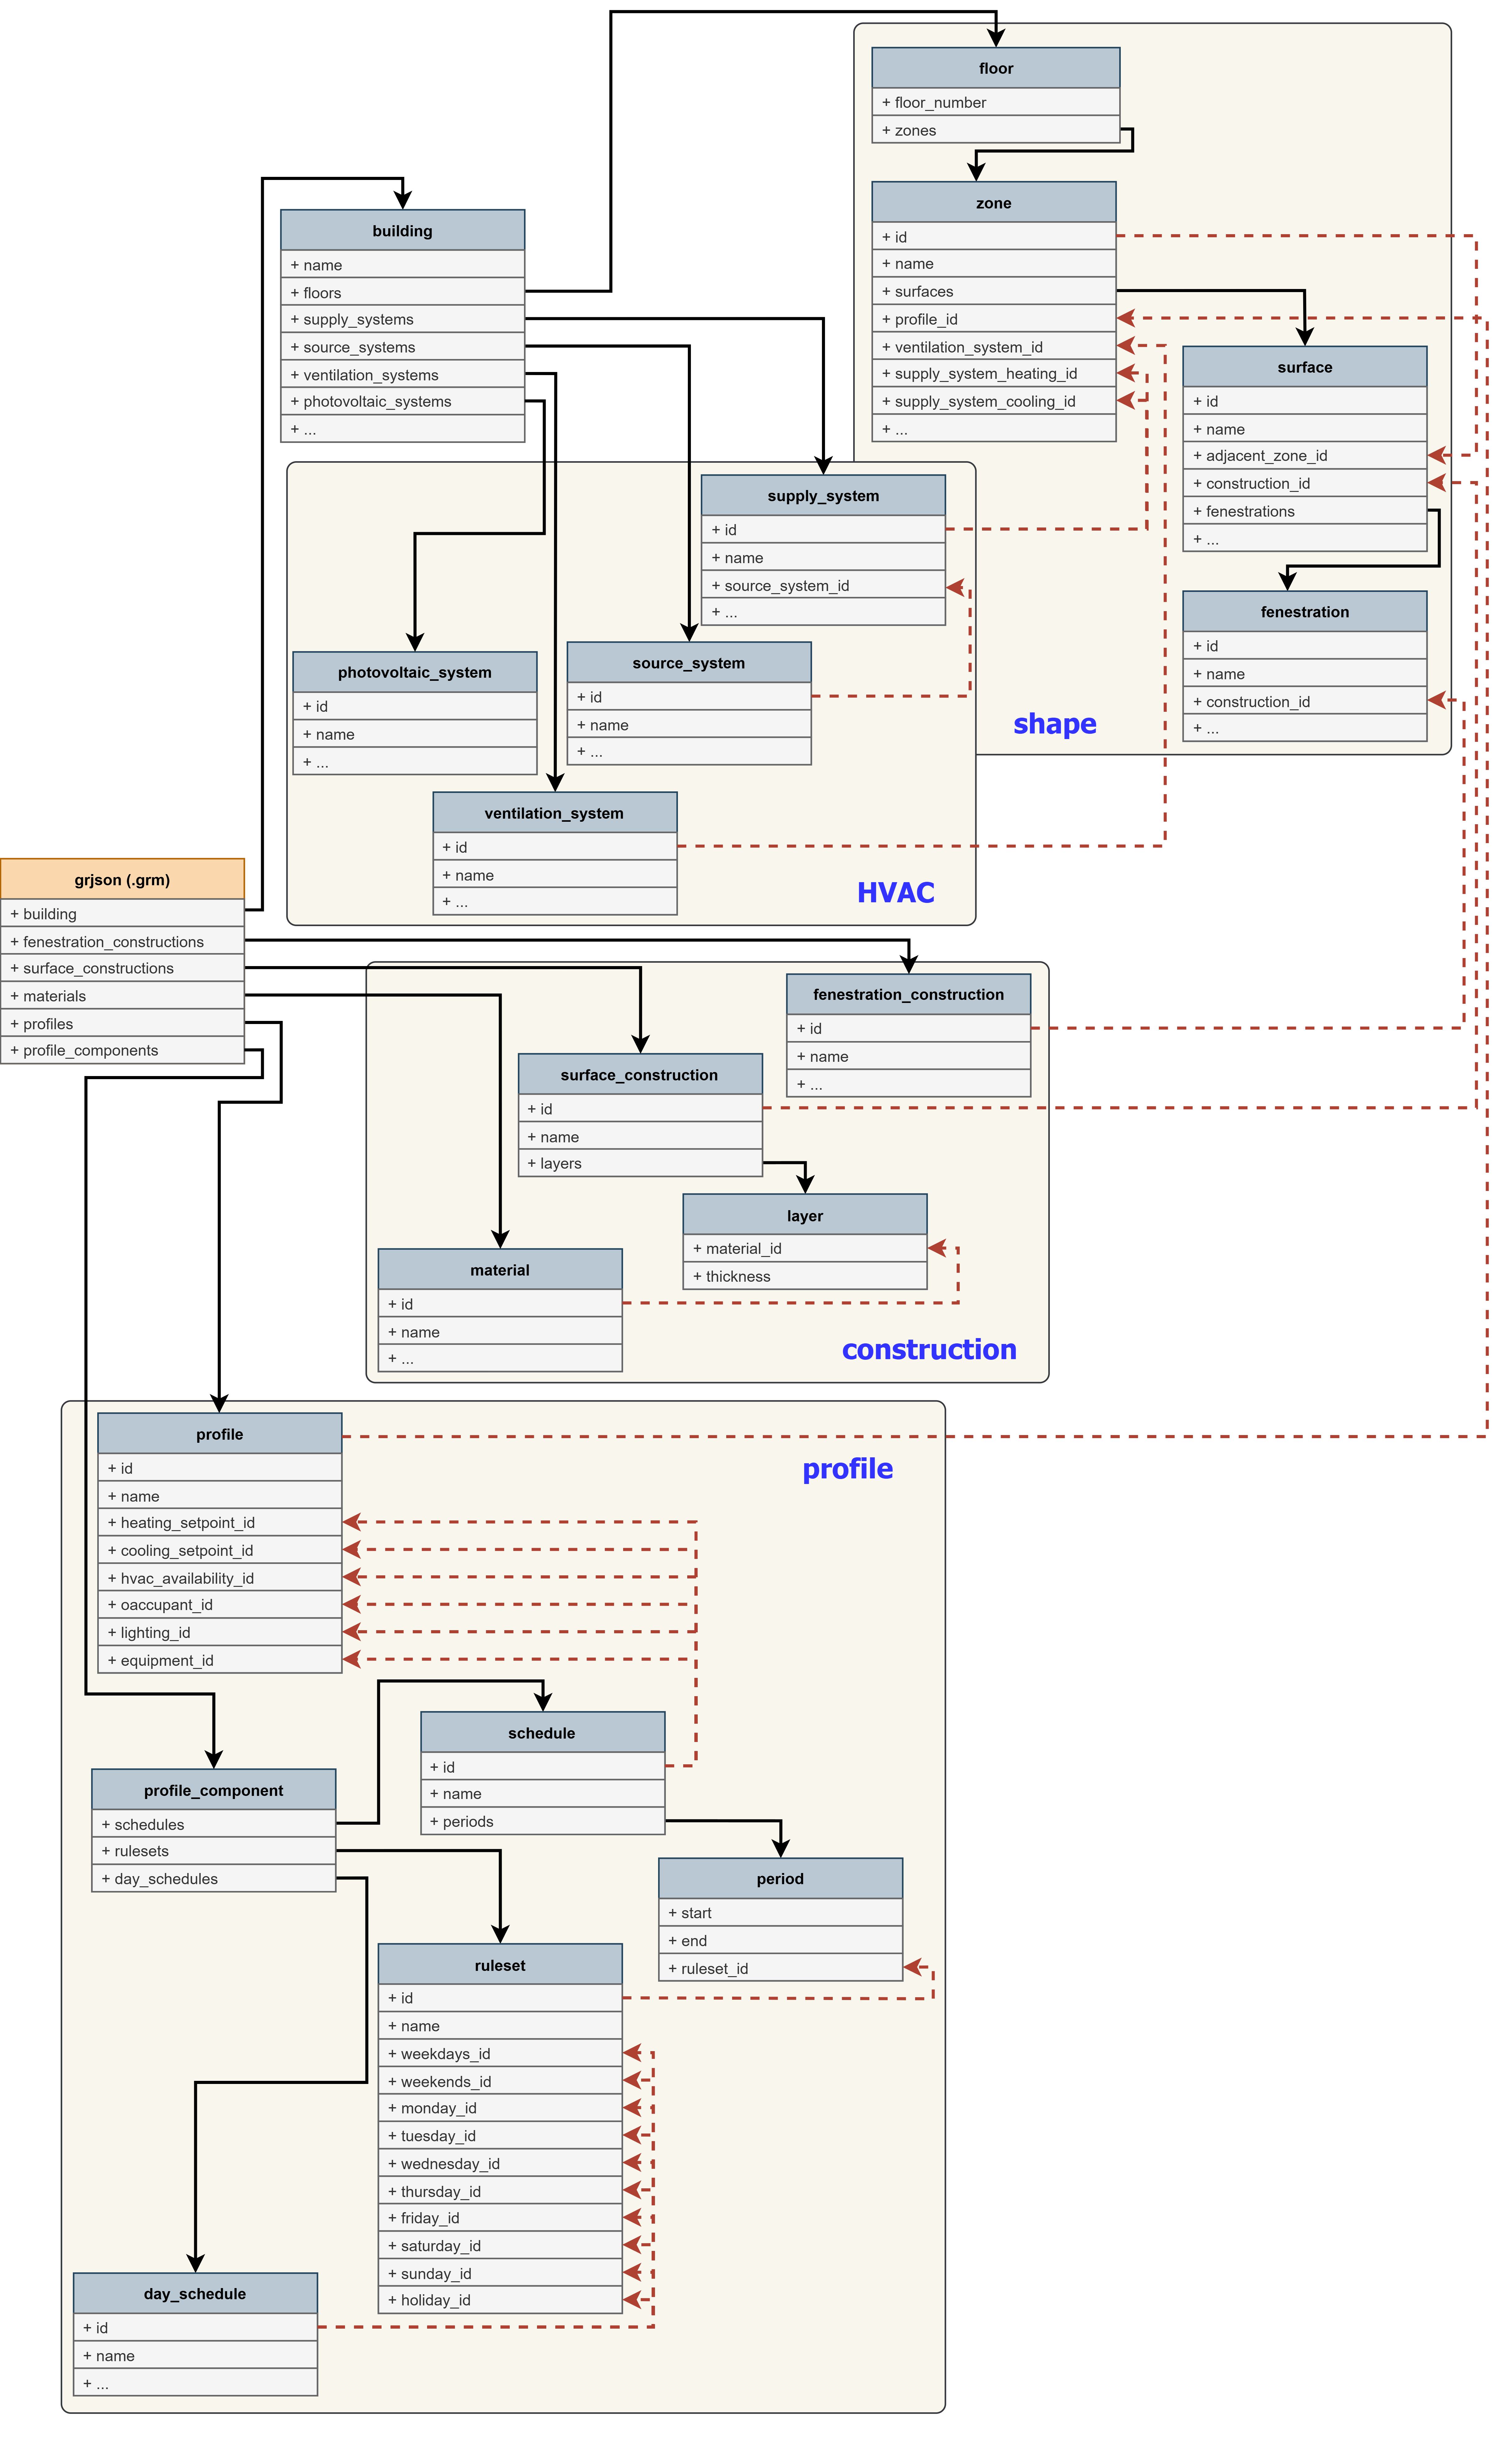
\includegraphics[height=0.99\textheight]{grjson_input_structure_v3.png}
  \caption{\simulator\ 입력변수 체계도}
  \label{fig:grjson_structure}
\end{defaultfigure}

% ---------------------------------------------------------------------------- %
%                                  NEW SECTION                                 %
% ---------------------------------------------------------------------------- %

\section{grjson 구조 (.grm 파일)}

\subsection{규칙}

\subsubsection{변수의 명칭 관련}

\paragraph{사용가능한 문자} 모든 변수의 명칭은 영문 소문자 및 밑줄(\_)로만 구성한다.

\paragraph{복수형과 단수형} 복수 객체 \texttt{array}를 담는 변수의 명칭(예: ``floors") 또는 복수 객체를 담는 하위 분류를 사용하는 변수의 명칭(예: ``profile\_components"), 길는 복수형을 사용하며, 단일 값을 담는 변수의 명칭(예: ``name")은 단수형을 사용한다. 단, 길이가 정해져있거나 각 위치별 의미가 명시적으로 다른 \texttt{array}를 담는 변수의 명칭(예: ``vintage")은 단수형을 사용한다.

\paragraph{축약형의 사용} 모든 변수의 명칭은 축약형을 사용하지 않는 것을 원칙으로 하되, 약어 자체로 통용되는 경우(예: ``cop\_heating")에는 축약형을 사용한다.

\subsubsection{ID 기반 객체 참조 관련} \label{subsubsection:ioref:id_description}
grjson에서 다른 객체의 지칭은 \texttt{ID}값에 기반하여 이루어지며, 모든 객체의 이름(``name")은 사용자 편의를 위한 이름으로 실제 데이터 변환 과정에서 사용되지 않는다.

\paragraph{사용가능한 문자} 모든 ID는 영문 대소문자, 숫자, 하이픈(-), 밑줄(\_)로만 구성되며, 숫자, 하이픈(-) 또는 밑줄(\_)로 시작하지 않는다.

\paragraph{ID의 중복} 동일한 \texttt{ID}는 같은 \texttt{class}의 객체끼리 공유할 수 없다. (모든 \texttt{class}에 대하여 서로 다른 \texttt{ID} 사용을 권장)

\subsubsection{변수의 유효성}

% ------------------------------- 여기서만 쓰는 함수들 ------------------------------- %

% --- 공통 chip (그대로 사용) ---
\newtcbox{\tagchip}[1][]{%
  on line, boxsep=0.6ex, left=0.9ex, right=0.9ex, top=0.2ex, bottom=0.2ex,
  arc=2.2pt, boxrule=0pt, colframe=white,
  colback=black, coltext=white, fontupper=\sffamily\bfseries\footnotesize,
  #1}

% --- 타입 색상 ---
\definecolor{typeString}{RGB}{206,145,120}
\definecolor{typeFloat}{RGB}{181,206,168}
\definecolor{typeInt}{RGB}{78,201,176}
\definecolor{typeEnum}{RGB}{86,156,214}
\definecolor{typeBool}{RGB}{142,206,221}

% --- 요구수준 색상 ---
\definecolor{reqBlueDark}{RGB}{37,99,235}
\definecolor{reqBlueLight}{RGB}{147,197,253}
\definecolor{reqGrayDark}{RGB}{107,114,128}
\definecolor{reqGrayLight}{RGB}{209,213,219}

% --- TypeTag (S/F/I/E) ---
\newcommand{\TypeTag}[1]{%
  \begingroup
  \ifthenelse{\equal{#1}{S}}{\tagchip[colback=typeString,coltext=black]{S}}{%
  \ifthenelse{\equal{#1}{F}}{\tagchip[colback=typeFloat ,coltext=black]{F}}{%
  \ifthenelse{\equal{#1}{I}}{\tagchip[colback=typeInt   ,coltext=white]{I}}{%
  \ifthenelse{\equal{#1}{E}}{\tagchip[colback=typeEnum  ,coltext=white]{E}}{%
  \ifthenelse{\equal{#1}{B}}{\tagchip[colback=typeBool  ,coltext=white]{B}}{%
  \tagchip[colback=gray!60,coltext=black]{#1}}}}}}%
  \endgroup
}

% --- ReqTag (R/CR/O/CO) ---
\newcommand{\ReqTag}[1]{%
  \begingroup
  \ifthenelse{\equal{#1}{R}} {\def\shade{reqBlueDark}\def\fg{white}}{}%
  \ifthenelse{\equal{#1}{CR}}{\def\shade{reqBlueLight}\def\fg{black}}{}%
  \ifthenelse{\equal{#1}{O}} {\def\shade{reqGrayDark}\def\fg{white}}{}%
  \ifthenelse{\equal{#1}{CO}}{\def\shade{reqGrayLight}\def\fg{black}}{}%
  \ifthenelse{\isundefined{\shade}}{\def\shade{gray!60}\def\fg{black}}{}%
  \tagchip[colback=\shade,coltext=\fg]{#1}%
  \endgroup
}

% --- table definition --- 
\newcommand{\jsontableunit}[1]{%
  \ifthenelse{\equal{#1}{}}{-}{$#1$}%
}

\newcommand{\jsontabledash}[1]{%
  \ifthenelse{\equal{#1}{}}{-}{#1}%
}

\newcommand{\jsontablerow}[7]{%
  \nolinkurl{#1} & #2 & #3 &
  \jsontabledash{#4} & \jsontabledash{#5} & \jsontabledash{#6} & \jsontableunit{#7} \\
}

\newcommand{\needtobeexplain}{상세설명 참고}

\newcommand{\jsontable}[2]{
  \begin{table}[htbp]
    \centering
    \caption{grjson 구조에서 \texttt{#1} 클래스의 속성들}
    {\footnotesize
    \begin{tabularx}{\textwidth}{l c c c Y Y c}
      \toprule
      변수명 & 타입 & 필수 & 기본값 & 조건 & 범위/길이/선택지 & 단위 \\
      \midrule
      #2
      \bottomrule
    \end{tabularx}
   } 
  \end{table}
}

모든 변수의 유효성은 필수 및 조건부 사용 여부에 따라 변수(의 속성) 값 존재의 유효성을 검사한 뒤, 타입 및 범위(또는 열거형 상수) 만족 여부를 검사하여 확인할 수 있다.

\paragraph{타입} 모든 변수는 정해진 타입의 변수여야 한다. 모든 변수의 타입은 문자\TypeTag{S}($String$), 실수\TypeTag{F}($Float$), 정수\TypeTag{I}($Integer$), 열거형\TypeTag{E}($Enum$), 불리언\TypeTag{B} 로 구분할 수 있다. 

\paragraph{필수 여부} 입력되지 않을 경우 에러가 발생하는 필수 변수\ReqTag{R}($Required$)와 달리, 비 필수 변수\ReqTag{O}($Optional$)는 미 입력 시 기본값이 사용된다. 단, 입력하지 않았다는 것을 명시적으로 \texttt{null}로 지정해야 하고, 변수 자체를 생락하면 안된다.

\paragraph{조건부 사용 여부} 어떤 변수는 다른 변수(주로 \texttt{type})의 값에 따라 조건부로 사용된다. 이 경우에도 해당 조건에서 필수적으로 요구되는 변수\ReqTag{CR}($Conditional Required$)와 그렇지 않은 변수\ReqTag{CO}($Conditional Optional$)로 구분할 수 있다. 조건에 만족하지 않는 경우, 해당 변수는 json에서 생략될 수 있다.

\paragraph{범위 및 열거형 상수} array면 길이 제약 따짐.
실수\TypeTag{F} 및 정수\TypeTag{I} 타입의 변수는 Python 부동소수점 및 정수 형식에서 표현 가능한 범위 내에서 처리된다.

\subsubsection{기타 규칙}

\paragraph{단위} 모든 변수는 SI 기본단위를 사용한다 (예: $m$, $J$, $W$, $kg$).

\subsection{class별 명세}

\subsubsection{building} \label{subsection:ioref:building}
실재하는 건물에 대한 최상위 정보 체계이다.

\jsontable{building}{
  \jsontablerow{name                 }{\TypeTag{S}}{\ReqTag{R}}{}{}{}{}
  \jsontablerow{north_axis           }{\TypeTag{F}}{\ReqTag{R}}{}{}{[0,360)}{deg(^\circ)}
  \jsontablerow{address              }{\TypeTag{S}}{\ReqTag{R}}{}{}{\needtobeexplain}{}
  \jsontablerow{vintage              }{[ \TypeTag{I} ]}{\ReqTag{R}}{}{}{[3,3]}{}
  \jsontablerow{num_aboveground_floor}{\TypeTag{I}}{\ReqTag{R}}{}{}{[1, $Inf$)}{}
  \jsontablerow{num_underground_floor}{\TypeTag{I}}{\ReqTag{R}}{}{}{[0, $Inf$)}{}
  \jsontablerow{floors               }{[ \hyperref[subsubsection:ioref:floor]{\texttt{floor}} ]}{}{}{}{[1, $Inf$)}{}
  \jsontablerow{supply_systems       }{[ \hyperref[subsubsection:ioref:supplysystem]{\texttt{supply\_system}} ]}{\ReqTag{R}}{}{}{[0, $Inf$)}{}
  \jsontablerow{source_systems       }{[ \hyperref[subsubsection:ioref:sourcesystem]{\texttt{source\_system}} ]}{\ReqTag{R}}{}{}{[0, $Inf$)}{}
  \jsontablerow{ventilation_systems  }{[ \hyperref[subsubsection:ioref:ventilationsystem]{\texttt{ventilation\_system}} ]}{\ReqTag{R}}{}{}{[0, $Inf$)}{}
  \jsontablerow{photovoltaic_systems }{[ \hyperref[subsubsection:ioref:photovoltaicsystem]{\texttt{photovoltaic\_system}} ]}{\ReqTag{R}}{}{}{[0, $Inf$)}{}
}

\paragraph{name} 건물의 이름. 시뮬레이션에 직접 사용되지 않는다.
\paragraph{north\_axis} 건물의 방위각. 도면상에서 나침반이 가리키는 방향 (반시계방향), 또는 건물의 향 관련 입력을 모두 회전시키는 동작 (시계방향) 을 지칭한다 (\cref{fig:ioref:north_axis}).

\begin{defaultfigure}
  
  \begin{subfigure}[b]{0.45\textwidth}
    \centering
    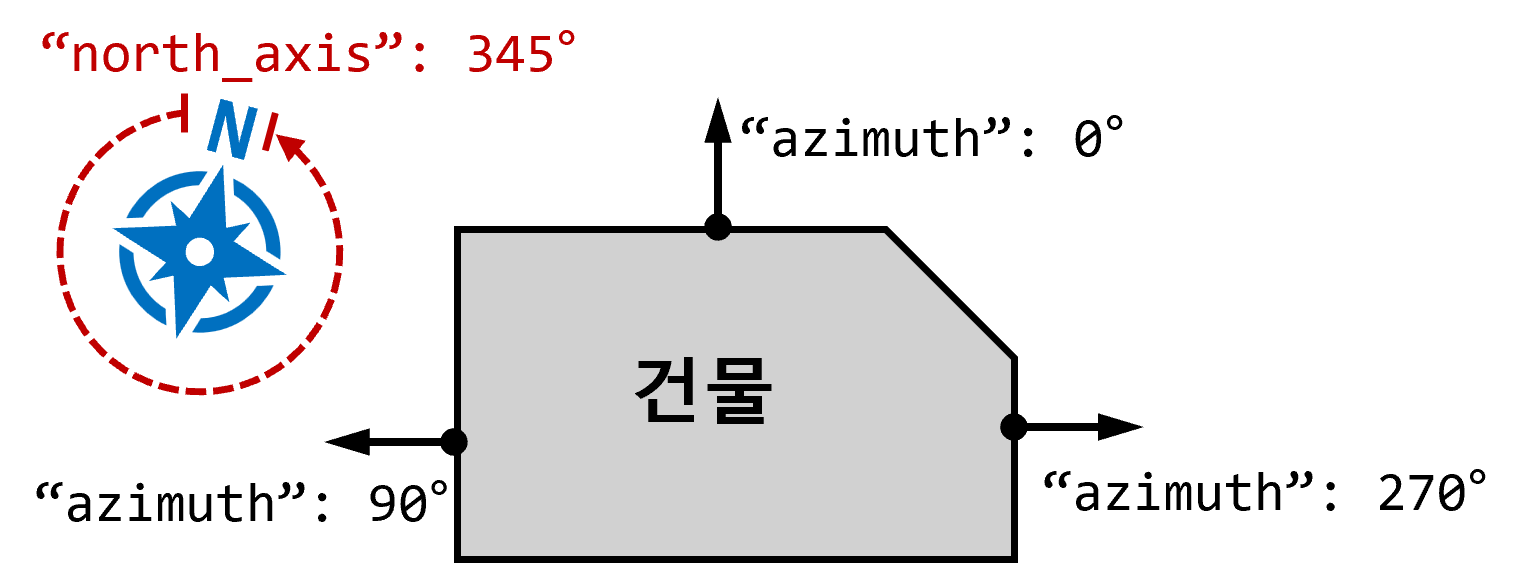
\includegraphics[scale=0.6]{north_axis 설명도식 (도면에서).png}
    \caption{도면에서}
  \end{subfigure}
  \hfill
  \begin{subfigure}[b]{0.45\textwidth}
    \centering
    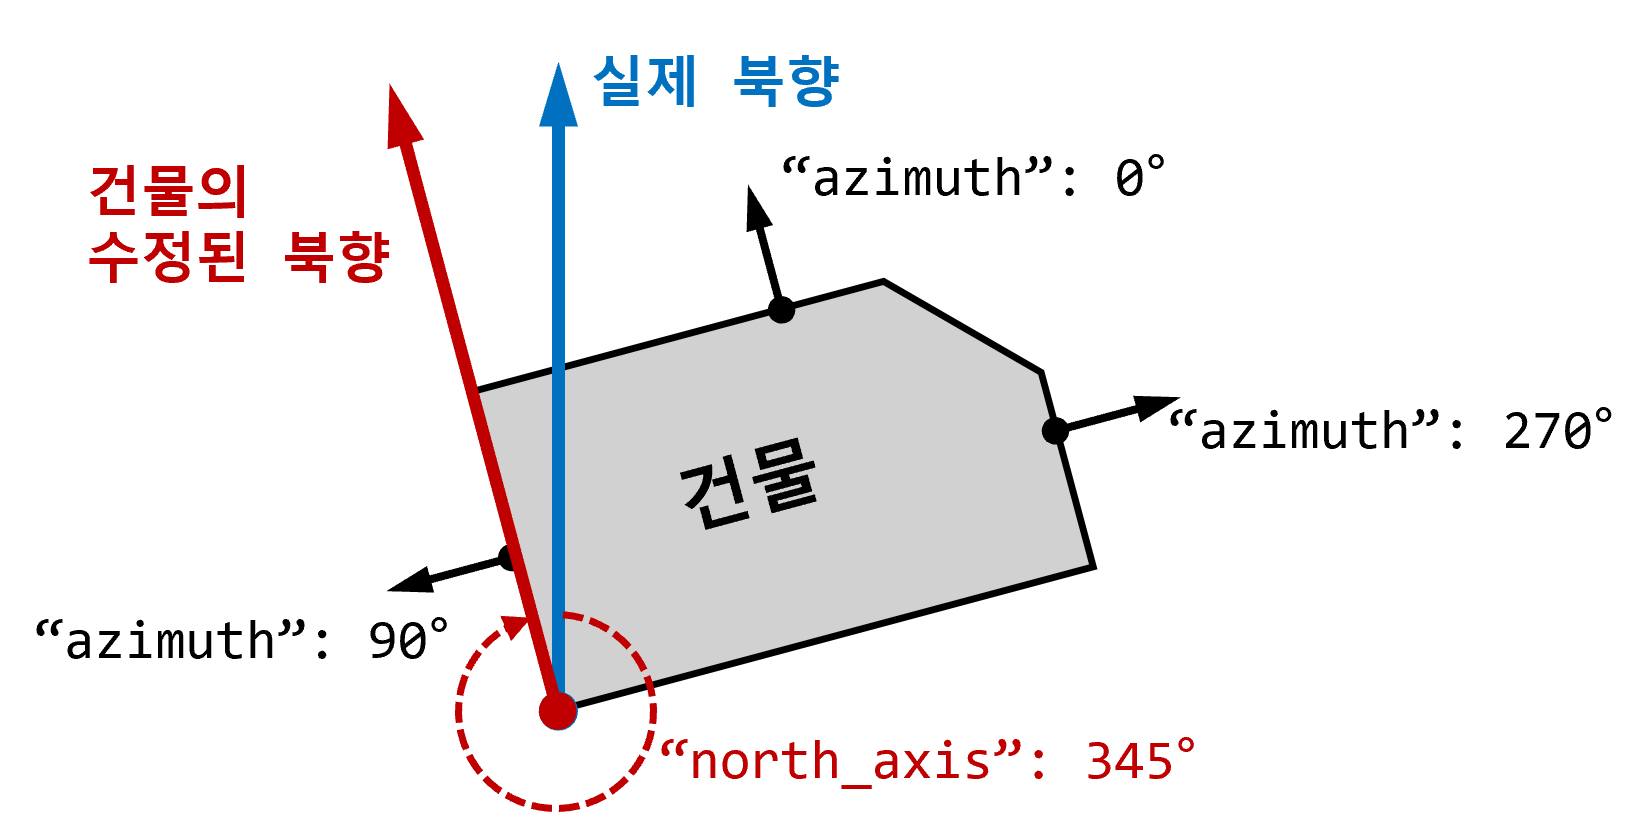
\includegraphics[scale=0.6]{north_axis 설명도식 (지도에서).png}
    \caption{지도에서}
  \end{subfigure}
  
  \caption{north\_axis의 의미와 surface azimuth와의 관계}
  \label{fig:ioref:north_axis}

\end{defaultfigure}

\paragraph{address} 건물의 주소. 식별 가능한 법정 기초행정구역명(세종특별자치시와 제주특별자치도 제주시, 서귀포시를 포함)을 포함하여야 한다. 

\paragraph{vintage} 건물의 허가일자. 연(4자리 정수), 월(2자리 정수), 일(2자리 정수)로 이루어진 array이다.

\paragraph{num\_aboveground\_floor} 건물의 지상 층 수. 시뮬레이션에 직접 사용되지 않는다.

\paragraph{num\_underground\_floor} 건물의 지하 층 수. 시뮬레이션에 직접 사용되지 않는다.

\subsubsection{floor} \label{subsubsection:ioref:floor}
하위 \hyperref[subsubsection:ioref:zone]{\texttt{zone}}들을 층 단위로 구분하기 위한 클래스이다.

\jsontable{floor}{
  \jsontablerow{floor_number}{\TypeTag{I}}{\ReqTag{O}}{0}{}{}{}
  \jsontablerow{zones}{[ \hyperref[subsubsection:ioref:zone]{\texttt{zone}} ]}{\ReqTag{R}}{}{}{[1,$Inf$)}{}
}

\paragraph{floor\_number} 층을 구별하기 위한 식별자. 시뮬레이션에 직접 사용되지 않는다.

\subsubsection{zone} \label{subsubsection:ioref:zone}
건물에서 하나의 실, 또는 같은 열적 특성(유사한 용도, 공통 설비 등)을 공유하는 서로 연결된 여러 실을 모사하는 최소 단위이다.

\jsontable{zone}{
  \jsontablerow{id                      }{\TypeTag{S}}{ \ReqTag{R} }{}{}{}{}
  \jsontablerow{name                    }{\TypeTag{S}}{ \ReqTag{R} }{}{}{}{}
  \jsontablerow{height                  }{\TypeTag{F}}{ \ReqTag{R} }{}{}{(0,$Inf$)}{m}
  \jsontablerow{profile                 }{\TypeTag{S}}{ \ReqTag{R} }{}{}{\needtobeexplain}{}
  \jsontablerow{profile_id              }{\TypeTag{S}}{ \ReqTag{CR}}{}{\texttt{profile} = ``custom''}{\hyperref[subsubsection:ioref:profile]{\texttt{profile}}의 \texttt{id}}{}
  \jsontablerow{light_density           }{\TypeTag{F}}{ \ReqTag{R} }{}{}{[0,$Inf$)}{W/m^{2}}
  \jsontablerow{infiltration            }{\TypeTag{F}}{ \ReqTag{R} }{}{}{[0,$Inf$)}{ACH50}
  \jsontablerow{supply_system_heating_id}{\TypeTag{S}}{ \ReqTag{R} }{}{}{\hyperref[subsubsection:ioref:supplysystem]{\texttt{supply\_system}}의 \texttt{id}}{}
  \jsontablerow{supply_system_cooling_id}{\TypeTag{S}}{ \ReqTag{R} }{}{}{\hyperref[subsubsection:ioref:supplysystem]{\texttt{supply\_system}}의 \texttt{id}}{}
  \jsontablerow{ventilation_system_id   }{\TypeTag{S}}{ \ReqTag{R} }{}{}{\hyperref[subsubsection:ioref:ventilationsystem]{\texttt{ventilation\_system}}의 \texttt{id}}{}
  \jsontablerow{surface                 }{[ \hyperref[subsubsection:ioref:surface]{\texttt{surface}} ]}{ \ReqTag{R} }{}{}{[0, $Inf$)}{}
}

\paragraph{id} 존의 식별자. \ref{subsubsection:ioref:id_description}에 따라 정의된다.

\paragraph{name} 사용자 편의를 위해 제공되는 존 구별 식별자. 중복, 사용가능한 문자에 제한이 없으며, 시뮬레이션에 직접 사용되지 않는다.

\paragraph{height} 존의 높이. 실의 부피 계산에 이용된다.

\paragraph{profile} 존의 용도프로필. 기본으로 제공되는 항목, 또는 ``custom'' 중에서 입력 가능하다. 

\paragraph{profile\_id} 존에 적용된 custom 용도프로필의 ID. 

\paragraph{light\_density} 조명 밀도.

\paragraph{supply\_system\_heating\_id} 난방공급시스템의 ID. 

\paragraph{supply\_system\_cooling\_id} 냉방공급시스템의 ID.

\paragraph{ventilation\_system\_id} 환기시스템의 ID.

\paragraph{surface} 소속면. 해당 \texttt{zone}을 인접존으로 하는 \texttt{surface}를 포함하여, 1개 이상의 천장(\texttt{type} = ``ceiling''), 1개 이상의 바닥(\texttt{type} = ``floor'') 및 1개 이상의 벽체(\texttt{type} = ``wall'')를 필요로 한다. 즉, 인접존이 없을 경우, 3 이상의 길이를 가지는 list가 필요하다.

\subsubsection{surface} \label{subsubsection:ioref:surface}
존과 존, 외부 (외기 또는 지면), 또는 단열선 사이의 면(벽체)이다.

\jsontable{surface}{
  \jsontablerow{id                  }{\TypeTag{S}}{\ReqTag{R} }{}{}{}{}
  \jsontablerow{name                }{\TypeTag{S}}{\ReqTag{R} }{}{}{}{}
  \jsontablerow{type                }{\TypeTag{E}}{\ReqTag{R} }{}{}{\shortstack[c]{floor \\ wall \\ ceiling}}{}
  \jsontablerow{boundary_condition  }{\TypeTag{E}}{\ReqTag{R} }{}{}{\shortstack[c]{outdoors \\zone \\ ground \\ adiabatic}}{}
  \jsontablerow{area                }{\TypeTag{F}}{\ReqTag{R} }{}{}{(0,$Inf$)}{m^2}
  \jsontablerow{azimuth             }{\TypeTag{F}}{\ReqTag{CR} }{}{\texttt{type} = ``wall'' \newline AND \newline \texttt{boundary\_condition} = ``outdoors''}{[0,360)}{deg(^\circ)}
  \jsontablerow{adjacent_zone_id    }{\TypeTag{S}}{\ReqTag{CR}}{}{\texttt{boundary\_condition} = ``zone''}{\hyperref[subsubsection:ioref:zone]{\texttt{zone}}의 \texttt{id}}{}
  \jsontablerow{construction_id     }{\TypeTag{S}}{\ReqTag{R}}{}{}{\hyperref[subsubsection:ioref:construction]{\texttt{construction}}의 \texttt{id} \newline ``open'' \newline ``unknown''}{}
  \jsontablerow{coolroof_reflectance}{\TypeTag{F}}{\ReqTag{CO}}{}{\texttt{type} = ``ceiling'' \newline AND \newline \texttt{boundary\_condition} = ``outdoors''}{(0,1]}{1}
  \jsontablerow{fenestrations       }{[ \hyperref[subsubsection:ioref:fenestration]{\texttt{fenestration}} ]}{\ReqTag{R}}{}{}{[0, $Inf$)}{}
}

\paragraph{id} 면의 식별자. \ref{subsubsection:ioref:id_description}에 따라 정의된다.

\paragraph{name} 사용자 편의를 위해 제공되는 면 구별 식별자. 중복, 사용가능한 문자에 제한이 없으며, 시뮬레이션에 직접 사용되지 않는다.

\paragraph{type} 면의 유형. 천장(``ceiling''), 바닥(``floor''), 벽체(``wall'')로 구분된다. 유형이 바닥(``floor'')인 면의 면적은 해당 \texttt{zone}의 면적에 포함되며, 유형이 천장(``ceiling'')인 면은 경계조건이 외기(``outdoors'')인 경우 쿨루프 적용이 가능하다.

\paragraph{boundary\_condition} 면의 경계조건. 일사와 바람의 영향을 받고 외기와 열교환을 하는 외기(``outdoors''), 다른 \texttt{zone}과 열교환을 하는 존(``zone''), 지면과 열교환을 하는 지면(``ground''), 어떠한 열교환도 하지 않고 축열의 역할만 담당하는 단열(``adiabatic'')로 구분된다 (Figure \ref{fig:surface_bo_description}).

\begin{defaultfigure}
  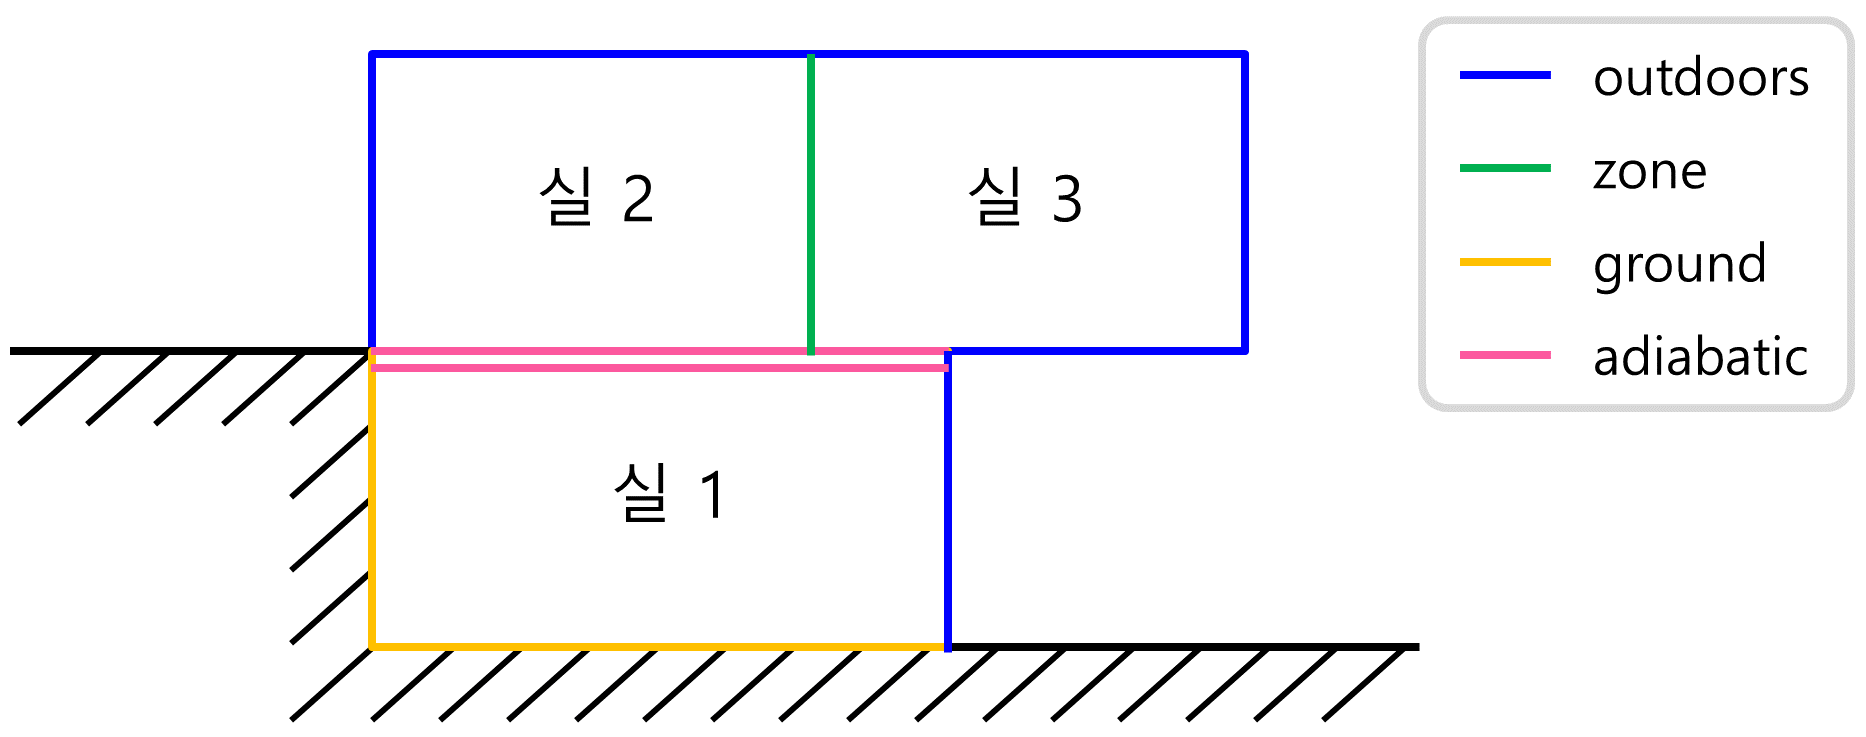
\includegraphics[width=0.8\textwidth]{면 경계조건 예시.png}
  \caption{면의 경계조건 예시}
  \label{fig:surface_bo_description}
\end{defaultfigure}

\paragraph{area} 면적. 해당 면에 개구부(예:창, 문 등)가 존재하는 경우, 이들의 면적을 포함한 전체 면적을 의미한다.

\paragraph{azimuth} 면의 방위각. 기준은 북향을 0$^\circ$로 하며, 반시계 방향으로 증가한다. 예를들어, 서향은 90$^\circ$, 남향은 180$^\circ$, 동쪽은 270$^\circ$로 정의한다.

\paragraph{adjacent\_zone\_id} 인접존 ID. 면의 경계조건을 ``zone''으로 설정한 경우에만 입력한다.

\paragraph{construction\_id} 구조체 ID. 

\paragraph{coolroof\_reflectance} 지붕면의 태양 반사율. 쿨루프(Cool Roof)시공이 적용된 경우에만 입력한다.

\subsubsection{fenestration} \label{subsubsection:ioref:fenestration}
개구부. 벽체의 열린 부분을 의미하며, 창, 문(유리문, 방화문 등) 등 외기와의 접촉 또는 채광·환기를 목적으로 설치된 요소를 포함한다.

\jsontable{fenestration}{
  \jsontablerow{id             }{\TypeTag{S}}{\ReqTag{R}}{}{}{}{}
  \jsontablerow{name           }{\TypeTag{S}}{\ReqTag{R}}{}{}{}{}
  \jsontablerow{type           }{\TypeTag{E}}{\ReqTag{R}}{}{}{\shortstack[c]{window \\ door \\ glassdoor}}{}
  \jsontablerow{area           }{\TypeTag{F}}{\ReqTag{R}}{}{}{(0,$Inf$)}{m^2}
  \jsontablerow{construction_id}{\TypeTag{S}}{\ReqTag{R}}{}{}{\hyperref[subsubsection:ioref:fenestrationconstruction]{\texttt{fenewtration\_construction}}의 \texttt{id}}{}
  \jsontablerow{blind          }{\TypeTag{E}}{\ReqTag{O}}{\texttt{null}}{}{\shortstack[c]{ venetian \\ shade}}{}
}

\paragraph{id} 개구부의 식별자. \ref{subsubsection:ioref:id_description}에 따라 정의된다.

\paragraph{name} 사용자 편의를 위해 제공되는 개구부 구별 식별자. 중복, 사용가능한 문자에 제한이 없으며, 시뮬레이션에 직접 사용되지 않는다.

\paragraph{type} 개구부의 유형. 유리창(``window''), 유리문(``glassdoor''), 또는 유리가 아닌 일반 문(``door'', 예: 방화문, 나무문 등)으로 구분된다.

\paragraph{area} 개구부의 면적. 해당 개구부가 속한 면의 면적보다 작아야 한다.

\paragraph{construction\_id} 개구부의 구조체. \texttt{type}이 ``window'' 또는 ``glassdoor''인 경우, \texttt{is\_transparent} 속성이 \texttt{True}인 구조체여야 한다. 반대로, \texttt{type}이 ``door''인 경우, \texttt{is\_transparent} 속성이 \texttt{False}인 구조체여야 한다

\paragraph{blind} 블라인드의 종류. 값이 \texttt{null}이면 블라인드가 없는 것을 의미한다.

\subsubsection{supply\_system} \label{subsubsection:ioref:supplysystem}
각 존에 존재하는 말단 공급설비이다. 

\jsontable{supply\_system}{
  \jsontablerow{id              }{\TypeTag{S}}{\ReqTag{R}}{}{}{}{}
  \jsontablerow{name            }{\TypeTag{S}}{\ReqTag{R}}{}{}{}{}
  \jsontablerow{type            }{\TypeTag{E}}{\ReqTag{R}}{}{}{\shortstack[c]{ packaged\_air\_conditioner \\ air\_handling\_unit \\ fan\_coil\_unit \\ radiator \\ electric\_radiator \\ radiant\_floor}}{}
  \jsontablerow{cop_cooling     }{\TypeTag{F}}{\ReqTag{CR}}{3.0}{\texttt{type} = ``packaged\_air\_conditioner''}{(0,$Inf$)}{W/W}
  \jsontablerow{capacity_cooling}{\TypeTag{F}}{\ReqTag{CR}}{\texttt{null}}{\texttt{type} = ``packaged\_air\_conditioner''}{(0,$Inf$)}{W}
  \jsontablerow{capacity_heating}{\TypeTag{F}}{\ReqTag{CR}}{\texttt{null}}{\texttt{type} = ``radiator'' OR ``electric\_radiator''}{(0,$Inf$)}{W}
  \jsontablerow{source_system_id}{\TypeTag{S}}{\ReqTag{CR}}{}{}{\hyperref[subsubsection:ioref:sourcesystem]{\texttt{source\_system}}의 \texttt{id}}{}
}

\paragraph{id} 공급설비의 식별자. \ref{subsubsection:ioref:id_description}에 따라 정의된다.

\paragraph{name} 사용자 편의를 위해 제공되는 공급설비 구별 식별자. 중복, 사용가능한 문자에 제한이 없으며, 시뮬레이션에 직접 사용되지 않는다.

\paragraph{type} 공급설비의 종류. 선택한 공급설비 유형에 따라 냉·난방 제공 가능 여부가 달라진다. 각 공급설비별 냉·난방 지원 가능 여부는 Figure \ref{fig:supply_and_source_properties_and_connection}에 제시되어 있다.

\paragraph{cop\_cooling} 정격 냉방 성능계수(COP). 정격 운전 조건에서의 냉방 출력을 소비 전력으로 나눈 값이다. 공급설비의 유형을 ``packaged\_airconditioner''로 선택한 경우에만 입력한다.

\paragraph{capacity\_cooling} 냉방용량. 설비의 최대 냉방 출력을 의미한다. 해당 값을 입력하지 않을 경우 (\texttt{null}), EnergyPlus의 autosizing을 이용한다. 공급설비의 유형을 ``packaged\_airconditioner''로 선택한 경우에만 입력한다.

\paragraph{capacity\_heating} 난방용량. 설비의 최대 난방 출력을 의미한다. 해당 값을 입력하지 않을 경우 (\texttt{null}), EnergyPlus의 autosizing을 이용한다. 공급설비의 유형을 ``radiator''혹은 ``electric\_radiator''로 선택한 경우에만 입력한다.

\paragraph{source\_system\_id} 연결된 생산설비의 ID. 연결가능한 생산설비는 Figure \ref{fig:supply_and_source_properties_and_connection}\와 같다.

\begin{defaultfigure}
  \includegraphics[width=\textwidth]{HVAC_properties_and_connectables.png}
  \caption{공급 및 생산설비 종류에 따른 요구 속성 및 연결 가능성 (적색 선은 난방, 청색 선은 냉방이 가능함을 의미하며, packaged\_air\_conditioner와 electric\_radiator는 생산설비의 연결을 요구하지 않는다.)}
  \label{fig:supply_and_source_properties_and_connection}
\end{defaultfigure}

\subsubsection{source\_system} \label{subsubsection:ioref:sourcesystem}
건물에 존재하는 생산설비이다.

\jsontable{source\_system}{
  \jsontablerow{id                   }{\TypeTag{S}}{\ReqTag{R} }{}{}{}{}
  \jsontablerow{name                 }{\TypeTag{S}}{\ReqTag{R} }{}{}{}{}
  \jsontablerow{type                 }{\TypeTag{E}}{\ReqTag{R} }{}{}{\shortstack[c]{ heatpump \\ geothermal\_heatpump \\ chiller \\ absorption\_chiller \\ boiler \\ district\_heating}}{}
  \jsontablerow{fuel_type            }{\TypeTag{E}}{\ReqTag{CR} }{}{\texttt{type} $\neq$ ``district\_heating''}{\shortstack[c]{electricity \\ natural\_gas \\ oil \\ district\_heating}}{}
  \jsontablerow{compressor_type      }{\TypeTag{E}}{\ReqTag{CR}}{}{\texttt{type} = ``chiller''}{\shortstack[c]{ turbo \\ screw \\ reciporating}}{}
  \jsontablerow{coolingtower_type    }{\TypeTag{E}}{\ReqTag{CR}}{}{\texttt{type} = ``chiller''}{\shortstack[c]{ closed \\ open}}{}
  \jsontablerow{coolingtower_control }{\TypeTag{E}}{\ReqTag{CR}}{}{\texttt{type} = ``chiller''}{\shortstack[c]{single-speed \\ two-speed}}{}
  \jsontablerow{hotwater_supply      }{\TypeTag{B}}{\ReqTag{CR}}{}{\texttt{type} = ``boiler'' OR ``district\_heating''}{}{}
  \jsontablerow{coolingtower_capacity}{\TypeTag{F}}{\ReqTag{CO}}{\texttt{null}}{\texttt{type} = ``chiller''}{(0, $Inf$)}{W}
  \jsontablerow{boiler_efficiency    }{\TypeTag{F}}{\ReqTag{CO}}{0.85}{\texttt{type} = ``absorption\_chiller''}{(0,1)}{1}
  \jsontablerow{capacity_cooling     }{\TypeTag{F}}{\ReqTag{CO}}{\texttt{null}}{\texttt{type} = ``chiller'' OR ``heatpump'' OR ``geothermal\_heatpump'' OR ``absorption\_chiller''}{(0,$Inf$)}{W}
  \jsontablerow{capacity_heating     }{\TypeTag{F}}{\ReqTag{CO}}{\texttt{null}}{\texttt{type} = ``heatpump'' OR ``geothermal\_heatpump'' OR ``boiler''}{(0,$Inf$)}{W}
  \jsontablerow{cop_cooling          }{\TypeTag{F}}{\ReqTag{CO}}{3.0}{\texttt{type} = ``heatpump'' OR ``geothermal\_heatpump'' OR ``absorption\_chiller''}{(0,$Inf$)}{W/W}
  \jsontablerow{cop_heating          }{\TypeTag{F}}{\ReqTag{CO}}{3.0}{\texttt{type} = ``heatpump'' OR ``geothermal\_heatpump''}{(0,$Inf$)}{W/W}
  \jsontablerow{efficiency           }{\TypeTag{F}}{\ReqTag{CO}}{0.85}{\texttt{type} = ``boiler''}{(0,1)}{1}
}

\paragraph{id} 생산설비의 식별자. \ref{subsubsection:ioref:id_description}에 따라 정의된다.

\paragraph{name} 사용자 편의를 위해 제공되는 생산설비 구별 식별자. 중복, 사용가능한 문자에 제한이 없으며, 시뮬레이션에 직접 사용되지 않는다.

\paragraph{type} 생산설비의 종류. 공급설비에 열을 제공하는 기기의 종류를 선택하며, 선택가능한 유형은 히트펌프(``heatpump''), 지열 히트펌프(``geothermal\_heatpump''), 칠러(``chiller''), 흡수식 칠러(``absorption\_chiller''), 보일러(``boiler''), 지역난방(``district\_heating'')이다.

\paragraph{fuel\_type} 연료의 종류. 생산설비의 사용 연료를 의미하며, 선택 가능한 항목은 전기(``electricity''), 천연가스/가스(``natural\_gas''), 난방유(``oil''), 지역난방(``district\_heating'')이다.

\paragraph{compressor\_type} 압축기의 종류. 

\paragraph{coolingtower\_type} 냉각탑의 종류. 

\paragraph{coolingtower\_control} 냉각탑에 적용된 제어. 

\paragraph{hotwater\_supply} 급탕공급 여부. 급탕을 공급하는 모든 생산설비들은 급탕효율 계산에 이용되며, 모든 설비가 동등하게 급탕 부하를 분담하는 것으로 가정한다.

\paragraph{coolingtower\_capacity} 냉각탑용량. 해당 값을 입력하지 않을 경우 (\texttt{null}) EnergyPlus의 autosizing을 이용한다.

\paragraph{boiler\_efficiency} 연동된 보일러의 효율.

\paragraph{capacity\_cooling} 냉방용량. 해당 값을 입력하지 않을 경우 (\texttt{null}) EnergyPlus의 autosizing을 이용한다.

\paragraph{capacity\_heating} 난방용량. 해당 값을 입력하지 않을 경우 (\texttt{null}) EnergyPlus의 autosizing을 이용한다.

\paragraph{cop\_cooling} 정격 냉방성능계수(COP). 정격 운전 조건에서의 냉방 출력을 소비 전력으로 나눈 값이다.

\paragraph{cop\_heating} 정격 난방성능계수(COP). 정격 운전 조건에서의 난방 출력을 소비 전력으로 나눈 값이다.

\paragraph{efficiency} 효율...

\subsubsection{ventilation\_system} \label{subsubsection:ioref:ventilationsystem}
환기설비다.

\jsontable{ventilation\_system}{
  \jsontablerow{id             }{\TypeTag{S}}{\ReqTag{R}}{}{}{}{}
  \jsontablerow{name           }{\TypeTag{S}}{\ReqTag{R}}{}{}{}{}
  \jsontablerow{efficiency_heating}{\TypeTag{F}}{\ReqTag{O}}{0.70}{}{(0,1)}{1}
  \jsontablerow{efficiency_cooling}{\TypeTag{F}}{\ReqTag{O}}{0.45}{}{(0,1)}{1}
}

\paragraph{id} 환기설비의 식별자. \ref{subsubsection:ioref:id_description}에 따라 정의된다.

\paragraph{name} 사용자 편의를 위해 제공되는 생산설비 구별 식별자. 중복, 사용가능한 문자에 제한이 없으며, 시뮬레이션에 직접 사용되지 않는다.

\paragraph{efficiency\_heating} 유효 냉방 전열교환 효율.

\paragraph{efficiency\_heating} 유효 난방 전열교환 효율.

\subsubsection{photovoltaic\_system} \label{subsubsection:ioref:photovoltaicsystem}
태양광 발전 설비.

\jsontable{photovoltaic\_system}{
  \jsontablerow{id        }{\TypeTag{S}}{\ReqTag{R}}{}{}{}{}
  \jsontablerow{name      }{\TypeTag{S}}{\ReqTag{R}}{}{}{}{}
  \jsontablerow{area      }{\TypeTag{F}}{\ReqTag{R}}{}{}{(0,$Inf$)}{m^2}
  \jsontablerow{azimuth   }{\TypeTag{F}}{\ReqTag{R}}{}{}{[0,360)}{deg(^\circ)}
  \jsontablerow{tilt      }{\TypeTag{F}}{\ReqTag{R}}{}{}{[0,90]}{deg(^\circ)}
  \jsontablerow{efficiency}{\TypeTag{F}}{\ReqTag{R}}{}{}{(0,1)}{1}
}

\paragraph{id} 태양광설비의 식별자. \ref{subsubsection:ioref:id_description}에 따라 정의된다.
 
\paragraph{name} 사용자 편의를 위해 제공되는 태양광설비 구별 식별자. 중복, 사용가능한 문자에 제한이 없으며, 시뮬레이션에 직접 사용되지 않는다.

\paragraph{area} 태양광 패널의 면적.

\paragraph{efficiency} 태양광 모듈의 발전 효율.

\paragraph{azimuth} 패널의 방위각. \hyperref[subsubsection:ioref:building]{\texttt{building}}의 \texttt{north\_axis}를 고려하지 않고 독립적으로 계산된다 (Figure \ref{fig:azimuth_of_PVpanel}). 

\begin{defaultfigure}
  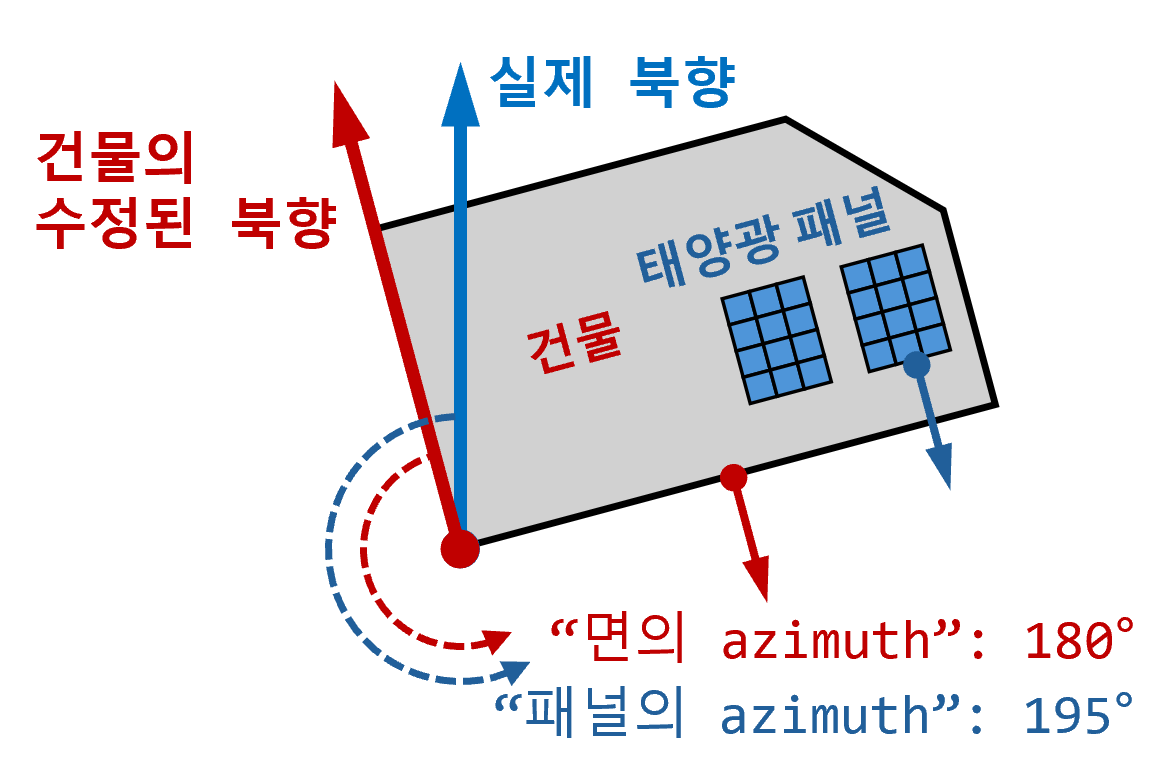
\includegraphics{태양광패널의 azimuth 설명.png}
  \caption{태양광 패널의 \texttt{azimuth}}
  \label{fig:azimuth_of_PVpanel}
\end{defaultfigure}

\paragraph{tilt} 패널의 경사각. 0$^\circ$는 수평면, 90$^\circ$는 수직면을 의미한다.

\subsubsection{profile} \label{subsubsection:ioref:profile}
존의 내부부하 및 발열을 나타내는 프로필이다.

\jsontable{profile}{
  \jsontablerow{id             }{\TypeTag{S}}{\ReqTag{R}}{}{}{}{}
  \jsontablerow{name           }{\TypeTag{S}}{\ReqTag{R}}{}{}{}{}
  \jsontablerow{hvac_availability_id}{\TypeTag{S}}{\ReqTag{R}}{}{}{\hyperref[subsubsection:ioref:schedule]{\texttt{schedule}}의 \texttt{id}}{}
  \jsontablerow{hotwater_id}{\TypeTag{S}}{\ReqTag{O}}{\texttt{null}}{}{\hyperref[subsubsection:ioref:schedule]{\texttt{schedule}}의 \texttt{id}}{}
  \jsontablerow{occupant_id}{\TypeTag{S}}{\ReqTag{O}}{\texttt{null}}{}{\hyperref[subsubsection:ioref:schedule]{\texttt{schedule}}의 \texttt{id}}{}
  \jsontablerow{lighting_id}{\TypeTag{S}}{\ReqTag{O}}{\texttt{null}}{}{\hyperref[subsubsection:ioref:schedule]{\texttt{schedule}}의 \texttt{id}}{}
  \jsontablerow{equipment_id}{\TypeTag{S}}{\ReqTag{O}}{\texttt{null}}{}{\hyperref[subsubsection:ioref:schedule]{\texttt{schedule}}의 \texttt{id}}{}
  \jsontablerow{heating_setpoint_id }{\TypeTag{S}}{\needtobeexplain}{\texttt{null}}{}{\hyperref[subsubsection:ioref:schedule]{\texttt{schedule}}의 \texttt{id}}{}
  \jsontablerow{cooling_setpoint_id }{\TypeTag{S}}{\needtobeexplain}{\texttt{null}}{}{\hyperref[subsubsection:ioref:schedule]{\texttt{schedule}}의 \texttt{id}}{}
}

\paragraph{id} 프로필의 식별자. \ref{subsubsection:ioref:id_description}에 따라 정의된다.

\paragraph{name} 사용자 편의를 위해 제공되는 프로필 구별 식별자. 중복, 사용가능한 문자에 제한이 없으며, 시뮬레이션에 직접 사용되지 않는다.

\paragraph{hvac\_availability\_id} 설비 운영 프로필의 식별자.

\paragraph{hotwater\_id} 급탕부하 스케줄. 해당 값을 입력하지 않을 경우 (\texttt{null}), 급탕부하가 없는 것으로 취급된다.

\paragraph{occupant\_id} 인체발열 스케줄. 해당 값을 입력하지 않을 경우 (\texttt{null}), 인체발열이 없는 것으로 취급된다.

\paragraph{lighting\_id} 조명발열 스케줄. 해당 값을 입력하지 않을 경우 (\texttt{null}), 조명발열이 없는 것으로 취급된다.

\paragraph{equipment\_id} 기기발열 스케줄. 해당 값을 입력하지 않을 경우 (\texttt{null}), 기기발열이 없는 것으로 취급된다.

\paragraph{heating\_setpoint\_id} 난방 설정온도 스케줄. 난방 설비를 가동하는 경우(\texttt{hvac\_availability\_id}의 모든 값이 0이 아닐 때)요구된다.

\paragraph{cooling\_setpoint\_id} 냉방 설정온도 스케줄. 냉방 설비를 가동하는 경우(\texttt{hvac\_availability\_id}의 모든 값이 0이 아닐 때)요구된다.

\subsubsection{profile\_component} \label{subsubsection:ioref:profile_component}
프로필을 구성하는 각 요소들(\texttt{scheduels},\texttt{rulesets},\texttt{day\_schedules})을 포함하는 개체이다.

\jsontable{profile\_component}{
  \jsontablerow{schedules    }{[ \hyperref[subsubsection:ioref:schedule]{\texttt{schedule}} ]}{\ReqTag{R}}{}{}{[0, $Inf$)}{}
  \jsontablerow{rulesets     }{[ \hyperref[subsubsection:ioref:ruleset]{\texttt{ruleset}} ]}{\ReqTag{R}}{}{}{[0, $Inf$)}{}
  \jsontablerow{day_schedules}{[ \hyperref[subsubsection:ioref:dayschedule]{\texttt{day\_schedule}} ]}{\ReqTag{R}}{}{}{[0, $Inf$)}{}
}

\subsubsection{schedule} \label{subsubsection:ioref:schedule}
ㅁㅁ
\jsontable{schedule}{
  \jsontablerow{id     }{\TypeTag{S}}{\ReqTag{R}}{}{}{}{}
  \jsontablerow{name   }{\TypeTag{S}}{\ReqTag{R}}{}{}{}{}
  \jsontablerow{periods}{[ \hyperref[subsubsection:ioref:period]{\texttt{period}} ]}{\ReqTag{R}}{}{}{}{}
}

\paragraph{id} 스케줄의 식별자. \ref{subsubsection:ioref:id_description}에 따라 정의된다.

\paragraph{name} 사용자 편의를 위해 제공되는 스케줄 구별 식별자. 중복, 사용가능한 문자에 제한이 없으며, 시뮬레이션에 직접 사용되지 않는다.

\subsubsection{period} \label{subsubsection:ioref:period}
주간 규칙을 적용할 기간을 명시한다.
\jsontable{period}{
  \jsontablerow{start     }{\TypeTag{S}}{\ReqTag{R}}{}{}{\needtobeexplain}{}
  \jsontablerow{end       }{\TypeTag{S}}{\ReqTag{R}}{}{}{\needtobeexplain}{}
  \jsontablerow{ruleset_id}{\TypeTag{S}}{\ReqTag{R}}{}{}{\hyperref[subsubsection:ioref:ruleset]{\texttt{ruleset}}의 \texttt{id}}{}
}

\paragraph{start} 기간이 시작하는 날짜. ``MM/DD''의 형태로 표기한다(예: 3월 17일 $\rightarrow$ ``03/17''). 참고로, 입력한 날짜는 기간에 포함된다.

\paragraph{end} 기간이 끝나는 날짜. ``MM/DD''의 형태로 표기한다(예: 3월 17일 $\rightarrow$ ``03/17''). 참고로, 입력한 날짜는 기간에 포함된다.

\paragraph{ruleset\_id} 적용할 주간 규칙의 ID.

\subsubsection{ruleset} \label{subsubsection:ioref:ruleset}
주간 규칙이다.
\jsontable{ruleset}{
  \jsontablerow{id          }{\TypeTag{S}}{\ReqTag{R}}{}{}{}{}
  \jsontablerow{name        }{\TypeTag{S}}{\ReqTag{R}}{}{}{}{}
  \jsontablerow{weekdays_id }{\TypeTag{S}}{\ReqTag{R}}{}{}{\hyperref[subsubsection:ioref:dayschedule]{\texttt{day\_schedule}}의 \texttt{id}}{}
  \jsontablerow{weekends_id }{\TypeTag{S}}{\ReqTag{R}}{}{}{\hyperref[subsubsection:ioref:dayschedule]{\texttt{day\_schedule}}의 \texttt{id}}{}
  \jsontablerow{monday_id   }{\TypeTag{S}}{\ReqTag{O}}{\texttt{null}}{}{\hyperref[subsubsection:ioref:dayschedule]{\texttt{day\_schedule}}의 \texttt{id}}{}
  \jsontablerow{tuesday_id  }{\TypeTag{S}}{\ReqTag{O}}{\texttt{null}}{}{\hyperref[subsubsection:ioref:dayschedule]{\texttt{day\_schedule}}의 \texttt{id}}{}
  \jsontablerow{wednesday_id}{\TypeTag{S}}{\ReqTag{O}}{\texttt{null}}{}{\hyperref[subsubsection:ioref:dayschedule]{\texttt{day\_schedule}}의 \texttt{id}}{}
  \jsontablerow{thursday_id }{\TypeTag{S}}{\ReqTag{O}}{\texttt{null}}{}{\hyperref[subsubsection:ioref:dayschedule]{\texttt{day\_schedule}}의 \texttt{id}}{}
  \jsontablerow{friday_id   }{\TypeTag{S}}{\ReqTag{O}}{\texttt{null}}{}{\hyperref[subsubsection:ioref:dayschedule]{\texttt{day\_schedule}}의 \texttt{id}}{}
  \jsontablerow{saturday_id }{\TypeTag{S}}{\ReqTag{O}}{\texttt{null}}{}{\hyperref[subsubsection:ioref:dayschedule]{\texttt{day\_schedule}}의 \texttt{id}}{}
  \jsontablerow{sunday_id   }{\TypeTag{S}}{\ReqTag{O}}{\texttt{null}}{}{\hyperref[subsubsection:ioref:dayschedule]{\texttt{day\_schedule}}의 \texttt{id}}{}
}

\paragraph{id} 주간규칙의 식별자. \ref{subsubsection:ioref:id_description}에 따라 정의된다.

\paragraph{name} 사용자 편의를 위해 제공되는 주간규칙 구별 식별자. 중복, 사용가능한 문자에 제한이 없으며, 시뮬레이션에 직접 사용되지 않는다.

\paragraph{weekdays\_id} 주중(월-금)에 적용되는 일간스케줄.

\paragraph{weekends\_id} 주말(토,일)에 적용되는 일간스케줄.

\paragraph{monday\_id} 월요일에 적용되는 일간스케줄. \texttt{null}이 아닌 경우, \texttt{weekdays\_id}보다 우선하여 적용된다.

\paragraph{tuesday\_id} 화요일에 적용되는 일간스케줄. \texttt{null}이 아닌 경우, \texttt{weekdays\_id}보다 우선하여 적용된다.

\paragraph{wednesday\_id} 수요일에 적용되는 일간스케줄. \texttt{null}이 아닌 경우, \texttt{weekdays\_id}보다 우선하여 적용된다.

\paragraph{thursday\_id} 목요일에 적용되는 일간스케줄. \texttt{null}이 아닌 경우, \texttt{weekdays\_id}보다 우선하여 적용된다.

\paragraph{friday\_id} 금요일에 적용되는 일간스케줄. \texttt{null}이 아닌 경우, \texttt{weekdays\_id}보다 우선하여 적용된다.

\paragraph{saturday\_id} 토요일에 적용되는 일간스케줄. \texttt{null}이 아닌 경우, \texttt{weekends\_id}보다 우선하여 적용된다.

\paragraph{sunday\_id} 일요일에 적용되는 일간스케줄. \texttt{null}이 아닌 경우, \texttt{weekends\_id}보다 우선하여 적용된다.

\paragraph{holiday\_id} 공휴일에 적용되는 일간스케줄. \texttt{null}인 경우, \texttt{sunday\_id}의 일간스케줄이 기본으로 적용된다.

\subsubsection{day\_schedule} \label{subsubsection:ioref:dayschedule}
일간스케줄이다.
\jsontable{day\_schedule}{
  \jsontablerow{id    }{\TypeTag{S}}{\ReqTag{R}}{}{}{}{}
  \jsontablerow{name  }{\TypeTag{S}}{\ReqTag{R}}{}{}{}{}
  \jsontablerow{type  }{\TypeTag{E}}{\ReqTag{R}}{}{}{}{}
  \jsontablerow{values}{[ \TypeTag{F} ]}{\ReqTag{R}}{}{}{144}{}
}

\paragraph{id} 일간스케줄의 식별자. \ref{subsubsection:ioref:id_description}에 따라 정의된다.

\paragraph{name} 사용자 편의를 위해 제공되는 일간스케줄 구별 식별자. 중복, 사용가능한 문자에 제한이 없으며, 시뮬레이션에 직접 사용되지 않는다.

\paragraph{type} 일간스케줄 종류. 시뮬레이션에 직접 사용되지 않는다.

\paragraph{values} 시간별 스케줄 값. 각 값은 10분간의 값을 의미하며, 크기가 144개인 시간별 값(array)로 입력한다(1일;24시간;1440분).

\subsubsection{material} \label{subsubsection:ioref:material}

\jsontable{material}{
  \jsontablerow{id           }{\TypeTag{S}}{\ReqTag{R}}{}{}{}{}
  \jsontablerow{name         }{\TypeTag{S}}{\ReqTag{R}}{}{}{}{}
  \jsontablerow{conductivity }{\TypeTag{F}}{\ReqTag{R}}{}{}{}{W{\cdot}m^{-1}{\cdot}K^{-1}}
  \jsontablerow{density      }{\TypeTag{F}}{\ReqTag{R}}{}{}{}{kg{\cdot}m^{-3}}
  \jsontablerow{specific_heat}{\TypeTag{F}}{\ReqTag{R}}{}{}{(100,$Inf$)}{J{\cdot}kg^{-1}{\cdot}K^{-1}}
}

\paragraph{id} 재료의 식별자. \ref{subsubsection:ioref:id_description}에 따라 정의된다.

\paragraph{name} 사용자 편의를 위해 제공되는 재료 구별 식별자. 중복, 사용가능한 문자에 제한이 없으며, 시뮬레이션에 직접 사용되지 않는다.

\paragraph{conductivity} 열전도율. 재료의 단위 두께를 통한 열 전달 능력을 나타낸다.

\paragraph{density} 밀도. 재료의 단위 부피당 질량을 나타낸다.

\paragraph{specific\_heat} 비열. 재료의 단위 질량이 1K 상승할 때 필요한 열량을 나타낸다.

\subsubsection{surface\_construction} \label{subsubsection:ioref:construction}

\jsontable{surface\_construction}{
  \jsontablerow{id    }{\TypeTag{S}}{\ReqTag{R}}{}{}{}{}
  \jsontablerow{name  }{\TypeTag{S}}{\ReqTag{R}}{}{}{}{}
  \jsontablerow{layers}{[ \hyperref[subsubsection:ioref:layer]{\texttt{layer}} ]}{\ReqTag{R}}{}{}{[1, 10]}{}
}
 
\paragraph{id} 레이어의 식별자. \ref{subsubsection:ioref:id_description}에 따라 정의된다.

\paragraph{name} 사용자 편의를 위해 제공되는 레이어 구별 식별자. 중복, 사용가능한 문자에 제한이 없으며, 시뮬레이션에 직접 사용되지 않는다.

\subsubsection{layer} \label{subsubsection:ioref:layer}

 \jsontable{layer}{
  \jsontablerow{material_id}{\TypeTag{S}}{\ReqTag{R}}{}{}{\hyperref[subsubsection:ioref:material]{\texttt{material}}의 \texttt{id}}{}
  \jsontablerow{thicknes   }{\TypeTag{F}}{\ReqTag{R}}{}{}{(0.003,$Inf$)}{m}
}

\paragraph{material\_id} 레이어 구성 재료의 ID.

\paragraph{thickness} 레이어 구성 재료의 두께.

\subsubsection{fenestration\_construction} \label{subsubsection:ioref:fenestrationconstruction}

\jsontable{fenestration\_construction}{
  \jsontablerow{id            }{\TypeTag{S}}{\ReqTag{R}}{}{}{}{}
  \jsontablerow{name          }{\TypeTag{S}}{\ReqTag{R}}{}{}{}{}
  \jsontablerow{is_transparent}{\TypeTag{B}}{\ReqTag{R}}{}{}{}{}
  \jsontablerow{u             }{\TypeTag{F}}{\ReqTag{R}}{}{}{(0, $Inf$)}{W{\cdot}m^{-1}{\cdot}K^{-1}}
  \jsontablerow{g             }{\TypeTag{F}}{\ReqTag{CR}}{}{\texttt{is\_transparent} = \texttt{True}}{(0,1]}{}
}

\paragraph{id} 창호의 식별자. \ref{subsubsection:ioref:id_description}에 따라 정의된다.

\paragraph{name} 사용자 편의를 위해 제공되는 창호 구별 식별자. 중복, 사용가능한 문자에 제한이 없으며, 시뮬레이션에 직접 사용되지 않는다.

\paragraph{is\_transparent} 구조체의 투명여부. 투명한 구조체의 개구부(예: 유리창, 유리문 등)는 ``True''로 입력하며, 불투명한 구조체의 개구부(예: 방화문, 나무문 등)는 ``False''로 입력한다.

\paragraph{u} 창호의 열관류율(U-value).

\paragraph{g} 창호의 열취득계수(G-value, SHGC).

% ---------------------------------------------------------------------------- %
%                                  NEW SECTION                                 %
% ---------------------------------------------------------------------------- %

\section{grexcel 구조 (.xlsx 파일)}
\subsection{개발규칙}
\texttt{grexcel}은 사용자에게 가장 친숙한 워크시트 도구인 Excel을 기반으로 
기본적인 데이터 입력 인터페이스(UI) 역할을 한다. 사용자가 한 페이지 내에서 많은 정보를 확인할 수 있도록 구성되어 있다.
\par
단위도 사용자에게 편한 단위 쓴다. 파란색은 수정 불가.. 초록색은 수정 가능한 영역을 나타내며 ...

\subsection{sheet별 명세}
\subsubsection{건물정보}

\subsubsection{실}

\subsubsection{면}

\subsubsection{개구부}

\subsubsection{구조체\_면}

\subsubsection{구조체\_개구부}

\subsubsection{구조체\_면}

\subsection{재료}

\subsection{공급설비}

\subsection{생산설비}

\subsection{환기설비}

\subsection{PV패널}

\subsection{예시}

\subsection{grexcel을 grjson으로 변환하는 과정}
아래 과정을 거쳐 변환된다.

유효한 컬럼만 남기기, 
컬럼명에서 단위 없애기, 
단위변환하기, 
값 변환하기, 
...

% ---------------------------------------------------------------------------- %
%                                  NEW SECTION                                 %
% ---------------------------------------------------------------------------- %

\section{grresult 구조 (.grr 파일)}
\subsection{class별 명세}
\subsubsection{입력정보 및 계산 방식 관련}
\paragraph{building} 건물 관련 기본 정보를 포함한다.
\begin{itemize}
  \item \textbf{total\_area}: 면적당 지표 계산에 사용되는 건물의 연면적($m^2$)을 의미한다. 연면적의 정의는 \ref{subsec:floorarea_definition_for_EUI}에서 기술한다.
\end{itemize}

\paragraph{constants} 연료별, 용도별, 월별 에너지소요량으로부터, 1차에너지소요량(site2source, $kWh/kWh$), 온실가스 배출량(site2co2, $kgCO_{2,eq}/kWh$) 및 에너지요금(site2cost, $won/kWh$)을 계산하는 데 사용된 변환계수를 포함한다. 각 변환계수의 산출 과정에 대하여는 \ref{subsec:result_converting_coeff_definition}에서 기술한다.

\subsubsection{원시데이터 관련}
에너지소요량을 비롯한 4가지 지표는 용도별 (6가지), 열원별 (4가지), 월별 (12개월)로 제시된다.
\begin{itemize}
  \item 6가지 용도: 난방(heating), 냉방(cooling), 조명(lighting), 팬/펌프/전열교환기(circulation), 급탕(hotwater), 발전(generators)
  \item 5가지 열원: 전기(ELECTRICITY), 천연가스(NATURALGAS), 등유(OIL), 지역난방(DISTRICTHEATING)
\end{itemize}

\paragraph{site\_uses} 건물에서 쓰는거 월별로 원별로 용도별로 제공한다.
\paragraph{source\_uses} 1차에너지에 해당된다. site\_uses에 계수를 곱해서 얻어진다.
\paragraph{co2} CO2 배출량이다. site\_uses에 계수를 곱해서 얻어진다.
\paragraph{cost} 비용이다. site\_uses에 계수를 곱해서 얻어진다.

\subsubsection{요약데이터 관련}
\paragraph{summary\_per\_area} 모두 합한 것이다.
\paragraph{summary\_gross} 에 면적을 곱한 것이다.

\subsection{예시}

아래는 결과 파일 예시이다.
